\documentclass[twoside]{book}

% Packages required by doxygen
\usepackage{fixltx2e}
\usepackage{calc}
\usepackage{doxygen}
\usepackage{graphicx}
\usepackage[utf8]{inputenc}
\usepackage{makeidx}
\usepackage{multicol}
\usepackage{multirow}
\PassOptionsToPackage{warn}{textcomp}
\usepackage{textcomp}
\usepackage[nointegrals]{wasysym}
\usepackage[table]{xcolor}

% Font selection
\usepackage[T1]{fontenc}
\usepackage{mathptmx}
\usepackage[scaled=.90]{helvet}
\usepackage{courier}
\usepackage{amssymb}
\usepackage{sectsty}
\renewcommand{\familydefault}{\sfdefault}
\allsectionsfont{%
  \fontseries{bc}\selectfont%
  \color{darkgray}%
}
\renewcommand{\DoxyLabelFont}{%
  \fontseries{bc}\selectfont%
  \color{darkgray}%
}
\newcommand{\+}{\discretionary{\mbox{\scriptsize$\hookleftarrow$}}{}{}}

% Page & text layout
\usepackage{geometry}
\geometry{%
  a4paper,%
  top=2.5cm,%
  bottom=2.5cm,%
  left=2.5cm,%
  right=2.5cm%
}
\tolerance=750
\hfuzz=15pt
\hbadness=750
\setlength{\emergencystretch}{15pt}
\setlength{\parindent}{0cm}
\setlength{\parskip}{0.2cm}
\makeatletter
\renewcommand{\paragraph}{%
  \@startsection{paragraph}{4}{0ex}{-1.0ex}{1.0ex}{%
    \normalfont\normalsize\bfseries\SS@parafont%
  }%
}
\renewcommand{\subparagraph}{%
  \@startsection{subparagraph}{5}{0ex}{-1.0ex}{1.0ex}{%
    \normalfont\normalsize\bfseries\SS@subparafont%
  }%
}
\makeatother

% Headers & footers
\usepackage{fancyhdr}
\pagestyle{fancyplain}
\fancyhead[LE]{\fancyplain{}{\bfseries\thepage}}
\fancyhead[CE]{\fancyplain{}{}}
\fancyhead[RE]{\fancyplain{}{\bfseries\leftmark}}
\fancyhead[LO]{\fancyplain{}{\bfseries\rightmark}}
\fancyhead[CO]{\fancyplain{}{}}
\fancyhead[RO]{\fancyplain{}{\bfseries\thepage}}
\fancyfoot[LE]{\fancyplain{}{}}
\fancyfoot[CE]{\fancyplain{}{}}
\fancyfoot[RE]{\fancyplain{}{\bfseries\scriptsize Generated on Sun Dec 21 2014 23\+:53\+:30 for My Project by Doxygen }}
\fancyfoot[LO]{\fancyplain{}{\bfseries\scriptsize Generated on Sun Dec 21 2014 23\+:53\+:30 for My Project by Doxygen }}
\fancyfoot[CO]{\fancyplain{}{}}
\fancyfoot[RO]{\fancyplain{}{}}
\renewcommand{\footrulewidth}{0.4pt}
\renewcommand{\chaptermark}[1]{%
  \markboth{#1}{}%
}
\renewcommand{\sectionmark}[1]{%
  \markright{\thesection\ #1}%
}

% Indices & bibliography
\usepackage{natbib}
\usepackage[titles]{tocloft}
\setcounter{tocdepth}{3}
\setcounter{secnumdepth}{5}
\makeindex

% Hyperlinks (required, but should be loaded last)
\usepackage{ifpdf}
\ifpdf
  \usepackage[pdftex,pagebackref=true]{hyperref}
\else
  \usepackage[ps2pdf,pagebackref=true]{hyperref}
\fi
\hypersetup{%
  colorlinks=true,%
  linkcolor=blue,%
  citecolor=blue,%
  unicode%
}

% Custom commands
\newcommand{\clearemptydoublepage}{%
  \newpage{\pagestyle{empty}\cleardoublepage}%
}


%===== C O N T E N T S =====

\begin{document}

% Titlepage & ToC
\hypersetup{pageanchor=false,
             bookmarks=true,
             bookmarksnumbered=true,
             pdfencoding=unicode
            }
\pagenumbering{roman}
\begin{titlepage}
\vspace*{7cm}
\begin{center}%
{\Large My Project }\\
\vspace*{1cm}
{\large Generated by Doxygen 1.8.8}\\
\vspace*{0.5cm}
{\small Sun Dec 21 2014 23:53:30}\\
\end{center}
\end{titlepage}
\clearemptydoublepage
\tableofcontents
\clearemptydoublepage
\pagenumbering{arabic}
\hypersetup{pageanchor=true}

%--- Begin generated contents ---
\chapter{Hierarchical Index}
\section{Class Hierarchy}
This inheritance list is sorted roughly, but not completely, alphabetically\+:\begin{DoxyCompactList}
\item \contentsline{section}{Application}{\pageref{class_application}}{}
\item \contentsline{section}{Camera}{\pageref{class_camera}}{}
\begin{DoxyCompactList}
\item \contentsline{section}{Camera2}{\pageref{class_camera2}}{}
\end{DoxyCompactList}
\item \contentsline{section}{Color}{\pageref{struct_color}}{}
\item \contentsline{section}{Component}{\pageref{struct_component}}{}
\item \contentsline{section}{Light}{\pageref{struct_light}}{}
\item \contentsline{section}{Material}{\pageref{struct_material}}{}
\item \contentsline{section}{Mesh}{\pageref{class_mesh}}{}
\item \contentsline{section}{Mesh\+Builder}{\pageref{class_mesh_builder}}{}
\item \contentsline{section}{Position}{\pageref{struct_position}}{}
\item \contentsline{section}{Scene}{\pageref{class_scene}}{}
\begin{DoxyCompactList}
\item \contentsline{section}{Scene1}{\pageref{class_scene1}}{}
\item \contentsline{section}{Scene2}{\pageref{class_scene2}}{}
\item \contentsline{section}{Scene3}{\pageref{class_scene3}}{}
\item \contentsline{section}{Scene4}{\pageref{class_scene4}}{}
\item \contentsline{section}{Scene5}{\pageref{class_scene5}}{}
\item \contentsline{section}{Scene\+Light}{\pageref{class_scene_light}}{}
\item \contentsline{section}{Scene\+Light2}{\pageref{class_scene_light2}}{}
\item \contentsline{section}{Scene\+Texture}{\pageref{class_scene_texture}}{}
\end{DoxyCompactList}
\item \contentsline{section}{Tex\+Coord}{\pageref{struct_tex_coord}}{}
\item \contentsline{section}{Vertex}{\pageref{struct_vertex}}{}
\end{DoxyCompactList}

\chapter{Class Index}
\section{Class List}
Here are the classes, structs, unions and interfaces with brief descriptions\+:\begin{DoxyCompactList}
\item\contentsline{section}{\hyperlink{class_application}{Application} \\*Provides methods to detect user input }{\pageref{class_application}}{}
\item\contentsline{section}{\hyperlink{class_camera}{Camera} \\*Provides to rotate around model to view it, but as it have issues \hyperlink{class_camera2}{Camera2} is generally preferred }{\pageref{class_camera}}{}
\item\contentsline{section}{\hyperlink{class_camera2}{Camera2} \\*Provides methods to rotate around model. This is preferred as it rotates around the model in a circle }{\pageref{class_camera2}}{}
\item\contentsline{section}{\hyperlink{struct_color}{Color} }{\pageref{struct_color}}{}
\item\contentsline{section}{\hyperlink{struct_component}{Component} \\*Provides methods to set the lighting of primitive shapes }{\pageref{struct_component}}{}
\item\contentsline{section}{\hyperlink{struct_light}{Light} \\*Provides methods to setup the light source }{\pageref{struct_light}}{}
\item\contentsline{section}{\hyperlink{struct_material}{Material} }{\pageref{struct_material}}{}
\item\contentsline{section}{\hyperlink{class_mesh}{Mesh} \\*To store V\+B\+O (vertex \& color buffer) and I\+B\+O (index buffer) }{\pageref{class_mesh}}{}
\item\contentsline{section}{\hyperlink{class_mesh_builder}{Mesh\+Builder} \\*Provides methods to generate mesh of different shapes }{\pageref{class_mesh_builder}}{}
\item\contentsline{section}{\hyperlink{struct_position}{Position} \\*Provides methods to set the color, position and vertex of primitive shapes }{\pageref{struct_position}}{}
\item\contentsline{section}{\hyperlink{class_scene}{Scene} \\*Provides methods to create other \hyperlink{class_scene}{Scene} classes, it is a an abstract class by itself }{\pageref{class_scene}}{}
\item\contentsline{section}{\hyperlink{class_scene1}{Scene1} }{\pageref{class_scene1}}{}
\item\contentsline{section}{\hyperlink{class_scene2}{Scene2} }{\pageref{class_scene2}}{}
\item\contentsline{section}{\hyperlink{class_scene3}{Scene3} }{\pageref{class_scene3}}{}
\item\contentsline{section}{\hyperlink{class_scene4}{Scene4} }{\pageref{class_scene4}}{}
\item\contentsline{section}{\hyperlink{class_scene5}{Scene5} }{\pageref{class_scene5}}{}
\item\contentsline{section}{\hyperlink{class_scene_light}{Scene\+Light} \\*Provides methods to create variables and functions to use for modelling }{\pageref{class_scene_light}}{}
\item\contentsline{section}{\hyperlink{class_scene_light2}{Scene\+Light2} }{\pageref{class_scene_light2}}{}
\item\contentsline{section}{\hyperlink{class_scene_texture}{Scene\+Texture} }{\pageref{class_scene_texture}}{}
\item\contentsline{section}{\hyperlink{struct_tex_coord}{Tex\+Coord} }{\pageref{struct_tex_coord}}{}
\item\contentsline{section}{\hyperlink{struct_vertex}{Vertex} }{\pageref{struct_vertex}}{}
\end{DoxyCompactList}

\chapter{File Index}
\section{File List}
Here is a list of all documented files with brief descriptions\+:\begin{DoxyCompactList}
\item\contentsline{section}{{\bfseries Application.\+h} }{\pageref{_application_8h}}{}
\item\contentsline{section}{{\bfseries Camera.\+h} }{\pageref{_camera_8h}}{}
\item\contentsline{section}{{\bfseries Camera2.\+h} }{\pageref{_camera2_8h}}{}
\item\contentsline{section}{{\bfseries Light.\+h} }{\pageref{_light_8h}}{}
\item\contentsline{section}{{\bfseries Material.\+h} }{\pageref{_material_8h}}{}
\item\contentsline{section}{{\bfseries Mesh.\+h} }{\pageref{_mesh_8h}}{}
\item\contentsline{section}{\hyperlink{_mesh_builder_8cpp}{Mesh\+Builder.\+cpp} \\*\hyperlink{_mesh_builder_8cpp}{Mesh\+Builder.\+cpp} is used to create the V\+B\+O and I\+B\+O of all primitive shapes }{\pageref{_mesh_builder_8cpp}}{}
\item\contentsline{section}{{\bfseries Mesh\+Builder.\+h} }{\pageref{_mesh_builder_8h}}{}
\item\contentsline{section}{{\bfseries Scene.\+h} }{\pageref{_scene_8h}}{}
\item\contentsline{section}{{\bfseries Scene1.\+h} }{\pageref{_scene1_8h}}{}
\item\contentsline{section}{{\bfseries Scene2.\+h} }{\pageref{_scene2_8h}}{}
\item\contentsline{section}{{\bfseries Scene3.\+h} }{\pageref{_scene3_8h}}{}
\item\contentsline{section}{{\bfseries Scene4.\+h} }{\pageref{_scene4_8h}}{}
\item\contentsline{section}{{\bfseries Scene5.\+h} }{\pageref{_scene5_8h}}{}
\item\contentsline{section}{\hyperlink{_scene_light_8cpp}{Scene\+Light.\+cpp} \\*\hyperlink{_mesh_builder_8h_source}{Mesh\+Builder.\+h} is used to set the function prototype for different shapes }{\pageref{_scene_light_8cpp}}{}
\item\contentsline{section}{{\bfseries Scene\+Light.\+h} }{\pageref{_scene_light_8h}}{}
\item\contentsline{section}{{\bfseries Scene\+Light2.\+h} }{\pageref{_scene_light2_8h}}{}
\item\contentsline{section}{{\bfseries shader.\+hpp} }{\pageref{shader_8hpp}}{}
\item\contentsline{section}{{\bfseries Utility.\+h} }{\pageref{_utility_8h}}{}
\item\contentsline{section}{{\bfseries Vertex.\+h} }{\pageref{_vertex_8h}}{}
\end{DoxyCompactList}

\chapter{Class Documentation}
\hypertarget{class_application}{\section{Application Class Reference}
\label{class_application}\index{Application@{Application}}
}


Provides methods to detect user input.  




{\ttfamily \#include $<$Application.\+h$>$}

\subsection*{Public Member Functions}
\begin{DoxyCompactItemize}
\item 
\hypertarget{class_application_a276388f7090c0a2b1c8b16cf033b969d}{void {\bfseries Init} ()}\label{class_application_a276388f7090c0a2b1c8b16cf033b969d}

\item 
\hypertarget{class_application_aaf09cd6cb412086dc039e28cdb059f0d}{void {\bfseries Run} ()}\label{class_application_aaf09cd6cb412086dc039e28cdb059f0d}

\item 
\hypertarget{class_application_a9d410604b39b8374a884b1f2a1f2a5ba}{void {\bfseries Exit} ()}\label{class_application_a9d410604b39b8374a884b1f2a1f2a5ba}

\end{DoxyCompactItemize}
\subsection*{Static Public Member Functions}
\begin{DoxyCompactItemize}
\item 
\hypertarget{class_application_a72cc9bba26506a7c0f54c346dfbd5cfe}{static bool {\bfseries Is\+Key\+Pressed} (unsigned short key)}\label{class_application_a72cc9bba26506a7c0f54c346dfbd5cfe}

\end{DoxyCompactItemize}


\subsection{Detailed Description}
Provides methods to detect user input. 

Class \hyperlink{class_application}{Application}\+: 

The documentation for this class was generated from the following files\+:\begin{DoxyCompactItemize}
\item 
Application.\+h\item 
Application.\+cpp\end{DoxyCompactItemize}

\hypertarget{class_camera}{\section{Camera Class Reference}
\label{class_camera}\index{Camera@{Camera}}
}


Provides to rotate around model to view it, but as it have issues \hyperlink{class_camera2}{Camera2} is generally preferred.  




{\ttfamily \#include $<$Camera.\+h$>$}

Inheritance diagram for Camera\+:\begin{figure}[H]
\begin{center}
\leavevmode
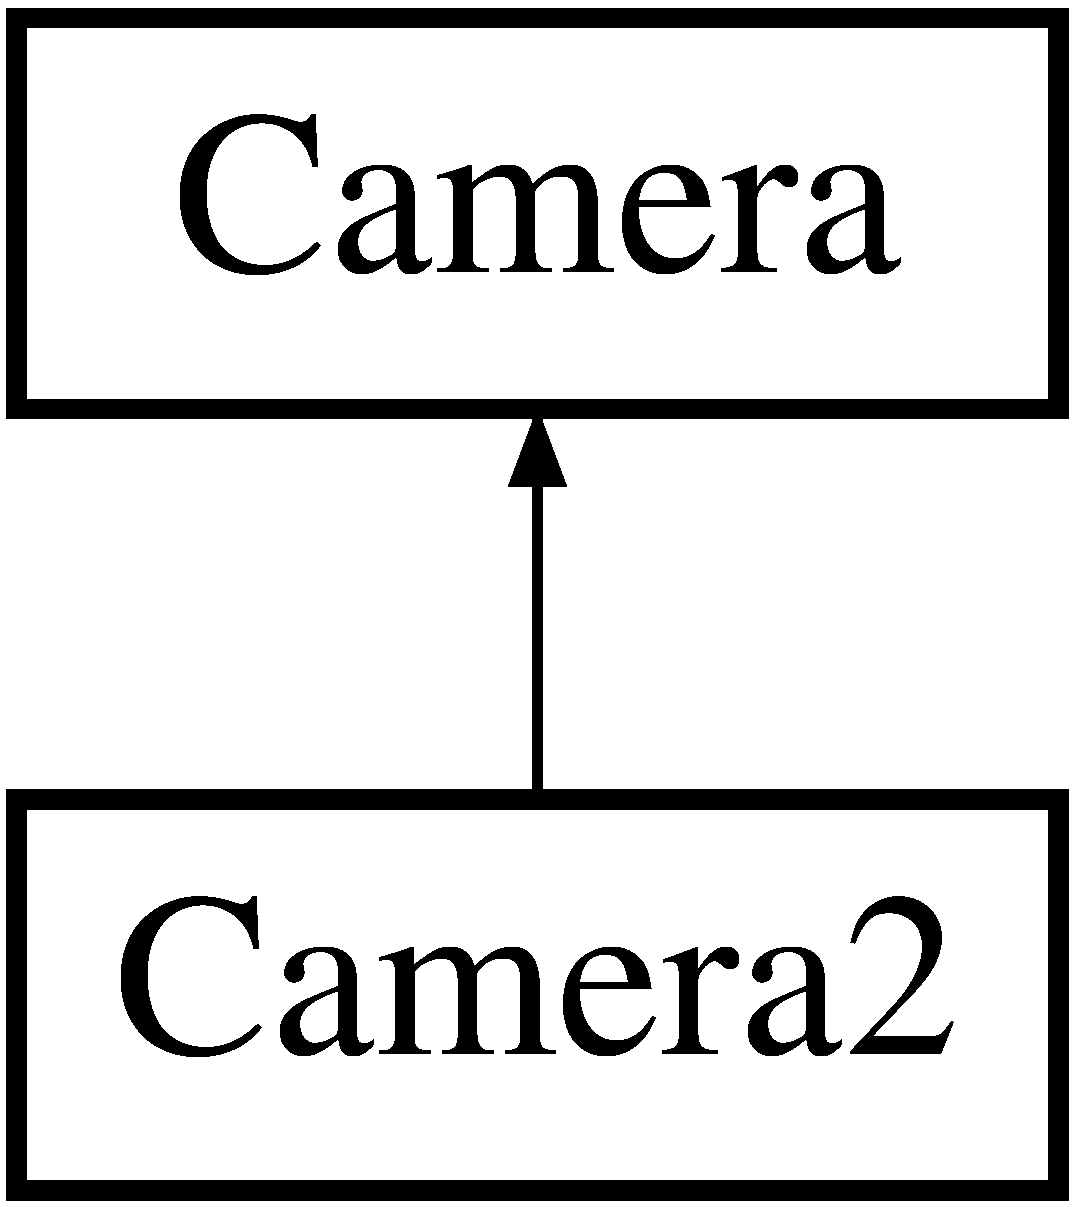
\includegraphics[height=2.000000cm]{class_camera}
\end{center}
\end{figure}
\subsection*{Public Member Functions}
\begin{DoxyCompactItemize}
\item 
\hypertarget{class_camera_a609775f7ec4cd936ad7add808cd7354c}{virtual void {\bfseries Init} (const Vector3 \&pos, const Vector3 \&target, const Vector3 \&up)}\label{class_camera_a609775f7ec4cd936ad7add808cd7354c}

\item 
\hypertarget{class_camera_aa46f58b32270a571ab56dde4caca46db}{virtual void {\bfseries Reset} ()}\label{class_camera_aa46f58b32270a571ab56dde4caca46db}

\item 
\hypertarget{class_camera_acc1741feb6d9da849ea4b6c12e0711e6}{virtual void {\bfseries Update} (double dt)}\label{class_camera_acc1741feb6d9da849ea4b6c12e0711e6}

\end{DoxyCompactItemize}
\subsection*{Public Attributes}
\begin{DoxyCompactItemize}
\item 
\hypertarget{class_camera_a3b229874a00253021a1b6c61657fa5ab}{Vector3 {\bfseries position}}\label{class_camera_a3b229874a00253021a1b6c61657fa5ab}

\item 
\hypertarget{class_camera_a7b1215b2f9c2a71cd41e4225c7df31e8}{Vector3 {\bfseries target}}\label{class_camera_a7b1215b2f9c2a71cd41e4225c7df31e8}

\item 
\hypertarget{class_camera_ab76ce866ca2acd6ab54447f474077245}{Vector3 {\bfseries up}}\label{class_camera_ab76ce866ca2acd6ab54447f474077245}

\end{DoxyCompactItemize}


\subsection{Detailed Description}
Provides to rotate around model to view it, but as it have issues \hyperlink{class_camera2}{Camera2} is generally preferred. 

Class \hyperlink{class_camera}{Camera}\+: 

The documentation for this class was generated from the following files\+:\begin{DoxyCompactItemize}
\item 
Camera.\+h\item 
Camera.\+cpp\end{DoxyCompactItemize}

\hypertarget{class_camera2}{\section{Camera2 Class Reference}
\label{class_camera2}\index{Camera2@{Camera2}}
}


Provides methods to rotate around model. This is preferred as it rotates around the model in a circle.  




{\ttfamily \#include $<$Camera2.\+h$>$}

Inheritance diagram for Camera2\+:\begin{figure}[H]
\begin{center}
\leavevmode
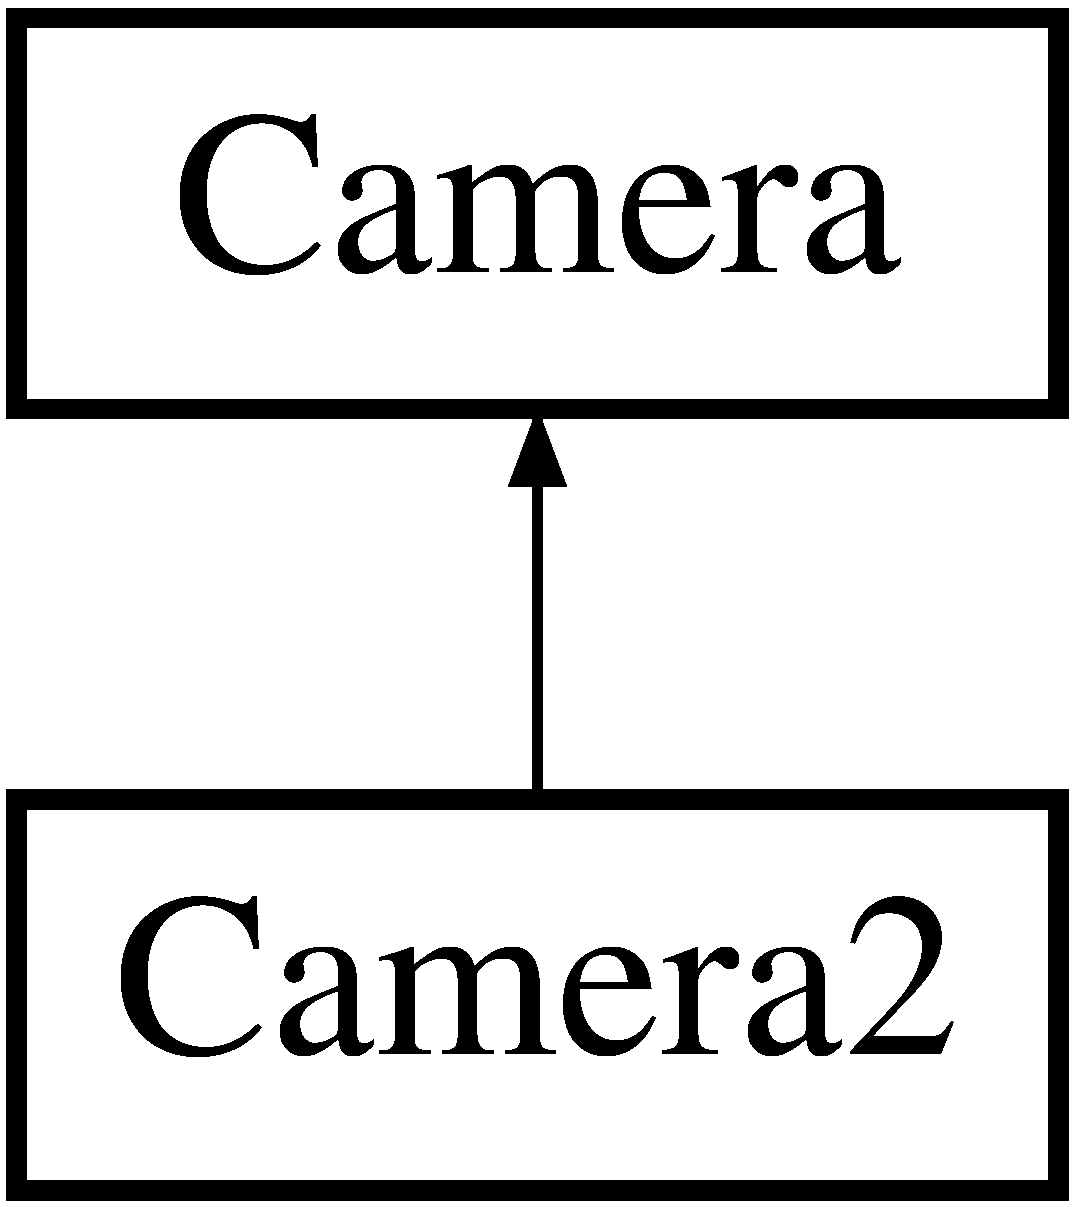
\includegraphics[height=2.000000cm]{class_camera2}
\end{center}
\end{figure}
\subsection*{Public Member Functions}
\begin{DoxyCompactItemize}
\item 
\hypertarget{class_camera2_af3d4e37be651bac9c0a94ac0af021c35}{virtual void {\bfseries Init} (const Vector3 \&pos, const Vector3 \&target, const Vector3 \&up)}\label{class_camera2_af3d4e37be651bac9c0a94ac0af021c35}

\item 
\hypertarget{class_camera2_a1a54eeb46692c8806b7abea38a6301f3}{virtual void {\bfseries Update} (double dt)}\label{class_camera2_a1a54eeb46692c8806b7abea38a6301f3}

\item 
\hypertarget{class_camera2_aeea4a4fb229742098c0f79cddbc19280}{virtual void {\bfseries Reset} ()}\label{class_camera2_aeea4a4fb229742098c0f79cddbc19280}

\end{DoxyCompactItemize}
\subsection*{Public Attributes}
\begin{DoxyCompactItemize}
\item 
\hypertarget{class_camera2_a248471e0c272cd78f83dcf18ff907c4f}{Vector3 {\bfseries default\+Position}}\label{class_camera2_a248471e0c272cd78f83dcf18ff907c4f}

\item 
\hypertarget{class_camera2_ab353b257dd3bee73e305205f5fe9b0c5}{Vector3 {\bfseries default\+Target}}\label{class_camera2_ab353b257dd3bee73e305205f5fe9b0c5}

\item 
\hypertarget{class_camera2_a2f700dc0fb49589a7f394be6f2152a7b}{Vector3 {\bfseries default\+Up}}\label{class_camera2_a2f700dc0fb49589a7f394be6f2152a7b}

\end{DoxyCompactItemize}


\subsection{Detailed Description}
Provides methods to rotate around model. This is preferred as it rotates around the model in a circle. 

Class \hyperlink{class_camera2}{Camera2}\+: 

The documentation for this class was generated from the following files\+:\begin{DoxyCompactItemize}
\item 
Camera2.\+h\item 
Camera2.\+cpp\end{DoxyCompactItemize}

\hypertarget{struct_color}{\section{Color Struct Reference}
\label{struct_color}\index{Color@{Color}}
}
\subsection*{Public Member Functions}
\begin{DoxyCompactItemize}
\item 
\hypertarget{struct_color_aa2ccdb977158b64bf8ad9000f443b09c}{{\bfseries Color} (float r=1, float g=1, float b=1)}\label{struct_color_aa2ccdb977158b64bf8ad9000f443b09c}

\item 
\hypertarget{struct_color_acc77e4e3583d3eca7e476952e51bfb80}{void {\bfseries Set} (float r, float g, float b)}\label{struct_color_acc77e4e3583d3eca7e476952e51bfb80}

\end{DoxyCompactItemize}
\subsection*{Public Attributes}
\begin{DoxyCompactItemize}
\item 
\hypertarget{struct_color_a3958a556b47d2de3dd45c75aac833c20}{float {\bfseries r}}\label{struct_color_a3958a556b47d2de3dd45c75aac833c20}

\item 
\hypertarget{struct_color_a5defbb21620e480e556181772d665f34}{float {\bfseries g}}\label{struct_color_a5defbb21620e480e556181772d665f34}

\item 
\hypertarget{struct_color_a33e482be18d6ea31d2b403bee13683b7}{float {\bfseries b}}\label{struct_color_a33e482be18d6ea31d2b403bee13683b7}

\end{DoxyCompactItemize}


The documentation for this struct was generated from the following file\+:\begin{DoxyCompactItemize}
\item 
Vertex.\+h\end{DoxyCompactItemize}

\hypertarget{struct_component}{\section{Component Struct Reference}
\label{struct_component}\index{Component@{Component}}
}


Provides methods to set the lighting of primitive shapes.  




{\ttfamily \#include $<$Material.\+h$>$}

\subsection*{Public Member Functions}
\begin{DoxyCompactItemize}
\item 
\hypertarget{struct_component_ae110a300786be861f7ea647ef77d9d18}{{\bfseries Component} (float r=0.\+1f, float g=0.\+1f, float b=0.\+1f)}\label{struct_component_ae110a300786be861f7ea647ef77d9d18}

\item 
\hypertarget{struct_component_a85f599b839327709953f0115dc5dfd49}{void {\bfseries Set} (float r, float g, float b)}\label{struct_component_a85f599b839327709953f0115dc5dfd49}

\end{DoxyCompactItemize}
\subsection*{Public Attributes}
\begin{DoxyCompactItemize}
\item 
\hypertarget{struct_component_a490db57cde183ef5a233b6ff3386ef6f}{float {\bfseries r}}\label{struct_component_a490db57cde183ef5a233b6ff3386ef6f}

\item 
\hypertarget{struct_component_a6cf7bfac62ac8aa4a8aa8c3f847428d8}{float {\bfseries g}}\label{struct_component_a6cf7bfac62ac8aa4a8aa8c3f847428d8}

\item 
\hypertarget{struct_component_abd55184abe2aaf269b38f5913721821c}{float {\bfseries b}}\label{struct_component_abd55184abe2aaf269b38f5913721821c}

\end{DoxyCompactItemize}


\subsection{Detailed Description}
Provides methods to set the lighting of primitive shapes. 

Class \hyperlink{struct_material}{Material}\+: 

The documentation for this struct was generated from the following file\+:\begin{DoxyCompactItemize}
\item 
Material.\+h\end{DoxyCompactItemize}

\hypertarget{struct_light}{\section{Light Struct Reference}
\label{struct_light}\index{Light@{Light}}
}


Provides methods to setup the light source.  




{\ttfamily \#include $<$Light.\+h$>$}

\subsection*{Public Attributes}
\begin{DoxyCompactItemize}
\item 
\hypertarget{struct_light_afeb738db41e987719e359166ef93314f}{\hyperlink{struct_position}{Position} {\bfseries position}}\label{struct_light_afeb738db41e987719e359166ef93314f}

\item 
\hypertarget{struct_light_ad7a168d26aed1bf7cca1a8d8e6f8ada4}{\hyperlink{struct_color}{Color} {\bfseries color}}\label{struct_light_ad7a168d26aed1bf7cca1a8d8e6f8ada4}

\item 
\hypertarget{struct_light_a6c4c401141c4cdb3b9b9b3bab7dd6fbb}{float {\bfseries power}}\label{struct_light_a6c4c401141c4cdb3b9b9b3bab7dd6fbb}

\item 
\hypertarget{struct_light_a888f11000d2baf1228d9e5c8d8c90fcb}{float {\bfseries k\+C}}\label{struct_light_a888f11000d2baf1228d9e5c8d8c90fcb}

\item 
\hypertarget{struct_light_ab3918c449fb40fa5c6cc5283f2c9687d}{float {\bfseries k\+L}}\label{struct_light_ab3918c449fb40fa5c6cc5283f2c9687d}

\item 
\hypertarget{struct_light_a79c8e47de58f131ff5403fc2d823cc21}{float {\bfseries k\+Q}}\label{struct_light_a79c8e47de58f131ff5403fc2d823cc21}

\end{DoxyCompactItemize}


\subsection{Detailed Description}
Provides methods to setup the light source. 

Class \hyperlink{struct_light}{Light}\+: 

The documentation for this struct was generated from the following file\+:\begin{DoxyCompactItemize}
\item 
Light.\+h\end{DoxyCompactItemize}

\hypertarget{struct_material}{\section{Material Struct Reference}
\label{struct_material}\index{Material@{Material}}
}
\subsection*{Public Attributes}
\begin{DoxyCompactItemize}
\item 
\hypertarget{struct_material_ab3819b3151cbf3ac1892195ab091e3b8}{\hyperlink{struct_component}{Component} {\bfseries k\+Ambient}}\label{struct_material_ab3819b3151cbf3ac1892195ab091e3b8}

\item 
\hypertarget{struct_material_aa88dd619cacf46e2f26ddd23fe032898}{\hyperlink{struct_component}{Component} {\bfseries k\+Diffuse}}\label{struct_material_aa88dd619cacf46e2f26ddd23fe032898}

\item 
\hypertarget{struct_material_a97cc0bf34b02c758b198d12dd24e96e2}{\hyperlink{struct_component}{Component} {\bfseries k\+Specular}}\label{struct_material_a97cc0bf34b02c758b198d12dd24e96e2}

\item 
\hypertarget{struct_material_a07cec8956c43f81adeb6ba7aea104915}{float {\bfseries k\+Shininess}}\label{struct_material_a07cec8956c43f81adeb6ba7aea104915}

\end{DoxyCompactItemize}


The documentation for this struct was generated from the following file\+:\begin{DoxyCompactItemize}
\item 
Material.\+h\end{DoxyCompactItemize}

\hypertarget{class_mesh}{\section{Mesh Class Reference}
\label{class_mesh}\index{Mesh@{Mesh}}
}


To store V\+B\+O (vertex \& color buffer) and I\+B\+O (index buffer)  




{\ttfamily \#include $<$Mesh.\+h$>$}

\subsection*{Public Types}
\begin{DoxyCompactItemize}
\item 
\hypertarget{class_mesh_a3d73fcae9980b9a36297a8481cf1a307}{enum {\bfseries D\+R\+A\+W\+\_\+\+M\+O\+D\+E} \{ {\bfseries D\+R\+A\+W\+\_\+\+T\+R\+I\+A\+N\+G\+L\+E\+S}, 
{\bfseries D\+R\+A\+W\+\_\+\+T\+R\+I\+A\+N\+G\+L\+E\+\_\+\+S\+T\+R\+I\+P}, 
{\bfseries D\+R\+A\+W\+\_\+\+L\+I\+N\+E\+S}, 
{\bfseries D\+R\+A\+W\+\_\+\+M\+O\+D\+E\+\_\+\+L\+A\+S\+T}
 \}}\label{class_mesh_a3d73fcae9980b9a36297a8481cf1a307}

\end{DoxyCompactItemize}
\subsection*{Public Member Functions}
\begin{DoxyCompactItemize}
\item 
\hyperlink{class_mesh_a8618160123ac2c27985d7ae34ad58cae}{Mesh} (const std\+::string \&mesh\+Name)
\begin{DoxyCompactList}\small\item\em Default constructor -\/ generate V\+B\+O/\+I\+B\+O here. \end{DoxyCompactList}\item 
\hypertarget{class_mesh_a5efe4da1a4c0971cfb037bd70304c303}{\hyperlink{class_mesh_a5efe4da1a4c0971cfb037bd70304c303}{$\sim$\+Mesh} ()}\label{class_mesh_a5efe4da1a4c0971cfb037bd70304c303}

\begin{DoxyCompactList}\small\item\em Destructor -\/ delete V\+B\+O/\+I\+B\+O here. \end{DoxyCompactList}\item 
\hypertarget{class_mesh_a75e66bcd90c09492676a4cfe5b23c3af}{void \hyperlink{class_mesh_a75e66bcd90c09492676a4cfe5b23c3af}{Render} ()}\label{class_mesh_a75e66bcd90c09492676a4cfe5b23c3af}

\begin{DoxyCompactList}\small\item\em Open\+G\+L render code. \end{DoxyCompactList}\end{DoxyCompactItemize}
\subsection*{Public Attributes}
\begin{DoxyCompactItemize}
\item 
\hypertarget{class_mesh_aa956ea809178c5713ca3e9220cee7980}{const std\+::string {\bfseries name}}\label{class_mesh_aa956ea809178c5713ca3e9220cee7980}

\item 
\hypertarget{class_mesh_ae12937ea9bdacb3b7b786f60fe42448e}{D\+R\+A\+W\+\_\+\+M\+O\+D\+E {\bfseries mode}}\label{class_mesh_ae12937ea9bdacb3b7b786f60fe42448e}

\item 
\hypertarget{class_mesh_a1e99394b36ad335804acd2461a736cfb}{unsigned {\bfseries vertex\+Buffer}}\label{class_mesh_a1e99394b36ad335804acd2461a736cfb}

\item 
\hypertarget{class_mesh_ad5efa4d45e469674dfa3765e479e4a73}{unsigned {\bfseries index\+Buffer}}\label{class_mesh_ad5efa4d45e469674dfa3765e479e4a73}

\item 
\hypertarget{class_mesh_ac6d6f70d161b9dd66c5ca79a187d86df}{unsigned {\bfseries index\+Size}}\label{class_mesh_ac6d6f70d161b9dd66c5ca79a187d86df}

\item 
\hypertarget{class_mesh_a7abd957a6487641e00c8fb855397bccd}{unsigned {\bfseries texture\+I\+D}}\label{class_mesh_a7abd957a6487641e00c8fb855397bccd}

\item 
\hypertarget{class_mesh_a3368c3bc60dd176e522df1542b764847}{\hyperlink{struct_material}{Material} {\bfseries material}}\label{class_mesh_a3368c3bc60dd176e522df1542b764847}

\end{DoxyCompactItemize}


\subsection{Detailed Description}
To store V\+B\+O (vertex \& color buffer) and I\+B\+O (index buffer) 

Class \hyperlink{class_mesh}{Mesh}\+: 

\subsection{Constructor \& Destructor Documentation}
\hypertarget{class_mesh_a8618160123ac2c27985d7ae34ad58cae}{\index{Mesh@{Mesh}!Mesh@{Mesh}}
\index{Mesh@{Mesh}!Mesh@{Mesh}}
\subsubsection[{Mesh}]{\setlength{\rightskip}{0pt plus 5cm}Mesh\+::\+Mesh (
\begin{DoxyParamCaption}
\item[{const std\+::string \&}]{mesh\+Name}
\end{DoxyParamCaption}
)}}\label{class_mesh_a8618160123ac2c27985d7ae34ad58cae}


Default constructor -\/ generate V\+B\+O/\+I\+B\+O here. 


\begin{DoxyParams}{Parameters}
{\em mesh\+Name} & -\/ name of mesh \\
\hline
\end{DoxyParams}


The documentation for this class was generated from the following files\+:\begin{DoxyCompactItemize}
\item 
Mesh.\+h\item 
Mesh.\+cpp\end{DoxyCompactItemize}

\hypertarget{class_mesh_builder}{\section{Mesh\+Builder Class Reference}
\label{class_mesh_builder}\index{Mesh\+Builder@{Mesh\+Builder}}
}


Provides methods to generate mesh of different shapes.  




{\ttfamily \#include $<$Mesh\+Builder.\+h$>$}

\subsection*{Static Public Member Functions}
\begin{DoxyCompactItemize}
\item 
static \hyperlink{class_mesh}{Mesh} $\ast$ \hyperlink{class_mesh_builder_a78d37e2b0cc068eec801f17c367100e7}{Generate\+Axes} (const std\+::string \&mesh\+Name, float length\+X, float length\+Y, float length\+Z)
\begin{DoxyCompactList}\small\item\em Generate the vertices of a reference Axes; Use red for x-\/axis, green for y-\/axis, blue for z-\/axis Then generate the V\+B\+O/\+I\+B\+O and store them in \hyperlink{class_mesh}{Mesh} object. \end{DoxyCompactList}\item 
static \hyperlink{class_mesh}{Mesh} $\ast$ \hyperlink{class_mesh_builder_aec661388bddf32e7bf834b38fb5ed34d}{Generate\+Quad} (const std\+::string \&mesh\+Name, \hyperlink{struct_color}{Color} color, float length)
\begin{DoxyCompactList}\small\item\em Generate the vertices of a quad; Use random color for each vertex Then generate the V\+B\+O/\+I\+B\+O and store them in \hyperlink{class_mesh}{Mesh} object. \end{DoxyCompactList}\item 
static \hyperlink{class_mesh}{Mesh} $\ast$ \hyperlink{class_mesh_builder_abe59149c68717536e3d638eb634b12e4}{Generate\+Triangle} (const std\+::string \&mesh\+Name, \hyperlink{struct_color}{Color} color, float length)
\begin{DoxyCompactList}\small\item\em Generate the vertices of a triangle; Then generate the V\+B\+O/\+I\+B\+O and store them in \hyperlink{class_mesh}{Mesh} object. \end{DoxyCompactList}\item 
static \hyperlink{class_mesh}{Mesh} $\ast$ \hyperlink{class_mesh_builder_a82d1778f4dc20e207d0e3158864c5f30}{Generate\+Cube} (const std\+::string \&mesh\+Name, \hyperlink{struct_color}{Color} color, float length=1.f)
\begin{DoxyCompactList}\small\item\em Generate the vertices of a cube; Use random color for each vertex Then generate the V\+B\+O/\+I\+B\+O and store them in \hyperlink{class_mesh}{Mesh} object. \end{DoxyCompactList}\item 
static \hyperlink{class_mesh}{Mesh} $\ast$ \hyperlink{class_mesh_builder_ab0c53a2d6f45d6cde847797839b3a2f5}{Generate\+Circle} (const std\+::string \&meshname, \hyperlink{struct_color}{Color} color, unsigned num\+Slice, float radius)
\begin{DoxyCompactList}\small\item\em Generate the vertices of a Circle; Then generate the V\+B\+O/\+I\+B\+O and store them in \hyperlink{class_mesh}{Mesh} object. \end{DoxyCompactList}\item 
static \hyperlink{class_mesh}{Mesh} $\ast$ \hyperlink{class_mesh_builder_a7bd766a7fb3be078327b66b271018e9e}{Generate\+Ring} (const std\+::string \&meshname, \hyperlink{struct_color}{Color} color, unsigned num\+Slice, float outer\+R, float inner\+R)
\begin{DoxyCompactList}\small\item\em Generate the vertices of a Ring; Then generate the V\+B\+O/\+I\+B\+O and store them in \hyperlink{class_mesh}{Mesh} object. \end{DoxyCompactList}\item 
static \hyperlink{class_mesh}{Mesh} $\ast$ \hyperlink{class_mesh_builder_a10f627b0355a031b42d0337e95d2af56}{Generate\+Sphere} (const std\+::string \&mesh\+Name, \hyperlink{struct_color}{Color} color, unsigned num\+Stack, unsigned num\+Slice, float radius)
\begin{DoxyCompactList}\small\item\em Generate the vertices of a Sphere; Then generate the V\+B\+O/\+I\+B\+O and store them in \hyperlink{class_mesh}{Mesh} object Functions called\+: sphere\+X, sphere\+Y, sphere\+Z. \end{DoxyCompactList}\item 
static \hyperlink{class_mesh}{Mesh} $\ast$ \hyperlink{class_mesh_builder_a0c4ccf0ee38c03b70cfe76443cacc543}{Generate\+Hemisphere} (const std\+::string \&mesh\+Name, \hyperlink{struct_color}{Color} color, unsigned num\+Stack, unsigned num\+Slice, float radius)
\begin{DoxyCompactList}\small\item\em Generate the vertices of a Hemisphere; Then generate the V\+B\+O/\+I\+B\+O and store them in \hyperlink{class_mesh}{Mesh} object Functions called\+: sphere\+X, sphere\+Y, sphere\+Z. \end{DoxyCompactList}\item 
static \hyperlink{class_mesh}{Mesh} $\ast$ \hyperlink{class_mesh_builder_a5829e4aa60902b040684c1d153c8ddf2}{Generate\+Cone} (const std\+::string \&meshname, \hyperlink{struct_color}{Color} color, unsigned num\+Slice, float radius, float height)
\begin{DoxyCompactList}\small\item\em Generate the vertices of a Cone; Then generate the V\+B\+O/\+I\+B\+O and store them in \hyperlink{class_mesh}{Mesh} object. \end{DoxyCompactList}\item 
static \hyperlink{class_mesh}{Mesh} $\ast$ \hyperlink{class_mesh_builder_ae32277cc64f8e2e94497331568fe610b}{Generate\+Cylinder} (const std\+::string \&mesh\+Name, \hyperlink{struct_color}{Color} color, unsigned num\+Stack, unsigned num\+Slice, unsigned stack\+Height, float height, float radius)
\begin{DoxyCompactList}\small\item\em Generate the vertices of a Cylinder; Then generate the V\+B\+O/\+I\+B\+O and store them in \hyperlink{class_mesh}{Mesh} object Functions called\+: Cylinder\+X, Cylinder\+Z. \end{DoxyCompactList}\end{DoxyCompactItemize}


\subsection{Detailed Description}
Provides methods to generate mesh of different shapes. 

Class \hyperlink{class_mesh_builder}{Mesh\+Builder}\+: 

\subsection{Member Function Documentation}
\hypertarget{class_mesh_builder_a78d37e2b0cc068eec801f17c367100e7}{\index{Mesh\+Builder@{Mesh\+Builder}!Generate\+Axes@{Generate\+Axes}}
\index{Generate\+Axes@{Generate\+Axes}!Mesh\+Builder@{Mesh\+Builder}}
\subsubsection[{Generate\+Axes}]{\setlength{\rightskip}{0pt plus 5cm}{\bf Mesh} $\ast$ Mesh\+Builder\+::\+Generate\+Axes (
\begin{DoxyParamCaption}
\item[{const std\+::string \&}]{mesh\+Name, }
\item[{float}]{length\+X, }
\item[{float}]{length\+Y, }
\item[{float}]{length\+Z}
\end{DoxyParamCaption}
)\hspace{0.3cm}{\ttfamily [static]}}}\label{class_mesh_builder_a78d37e2b0cc068eec801f17c367100e7}


Generate the vertices of a reference Axes; Use red for x-\/axis, green for y-\/axis, blue for z-\/axis Then generate the V\+B\+O/\+I\+B\+O and store them in \hyperlink{class_mesh}{Mesh} object. 


\begin{DoxyParams}{Parameters}
{\em mesh\+Name} & -\/ name of mesh \\
\hline
{\em length\+X} & -\/ x-\/axis should start at -\/length\+X / 2 and end at length\+X / 2 \\
\hline
{\em length\+Y} & -\/ y-\/axis should start at -\/length\+Y / 2 and end at length\+Y / 2 \\
\hline
{\em length\+Z} & -\/ z-\/axis should start at -\/length\+Z / 2 and end at length\+Z / 2\\
\hline
\end{DoxyParams}
\begin{DoxyReturn}{Returns}
Pointer to mesh storing V\+B\+O/\+I\+B\+O of reference axes 
\end{DoxyReturn}
\hypertarget{class_mesh_builder_ab0c53a2d6f45d6cde847797839b3a2f5}{\index{Mesh\+Builder@{Mesh\+Builder}!Generate\+Circle@{Generate\+Circle}}
\index{Generate\+Circle@{Generate\+Circle}!Mesh\+Builder@{Mesh\+Builder}}
\subsubsection[{Generate\+Circle}]{\setlength{\rightskip}{0pt plus 5cm}{\bf Mesh} $\ast$ Mesh\+Builder\+::\+Generate\+Circle (
\begin{DoxyParamCaption}
\item[{const std\+::string \&}]{mesh\+Name, }
\item[{{\bf Color}}]{color, }
\item[{unsigned}]{num\+Slice, }
\item[{float}]{radius}
\end{DoxyParamCaption}
)\hspace{0.3cm}{\ttfamily [static]}}}\label{class_mesh_builder_ab0c53a2d6f45d6cde847797839b3a2f5}


Generate the vertices of a Circle; Then generate the V\+B\+O/\+I\+B\+O and store them in \hyperlink{class_mesh}{Mesh} object. 


\begin{DoxyParams}{Parameters}
{\em mesh\+Name} & -\/ name of mesh \\
\hline
{\em color} & -\/ set color \\
\hline
{\em num\+Slice} & -\/ set the Index buffer data \\
\hline
{\em radius} & -\/ set the radius of triangle\\
\hline
\end{DoxyParams}
\begin{DoxyReturn}{Returns}
Pointer to mesh storing V\+B\+O/\+I\+B\+O of reference axes 
\end{DoxyReturn}
\hypertarget{class_mesh_builder_a5829e4aa60902b040684c1d153c8ddf2}{\index{Mesh\+Builder@{Mesh\+Builder}!Generate\+Cone@{Generate\+Cone}}
\index{Generate\+Cone@{Generate\+Cone}!Mesh\+Builder@{Mesh\+Builder}}
\subsubsection[{Generate\+Cone}]{\setlength{\rightskip}{0pt plus 5cm}{\bf Mesh} $\ast$ Mesh\+Builder\+::\+Generate\+Cone (
\begin{DoxyParamCaption}
\item[{const std\+::string \&}]{mesh\+Name, }
\item[{{\bf Color}}]{color, }
\item[{unsigned}]{num\+Slice, }
\item[{float}]{radius, }
\item[{float}]{height}
\end{DoxyParamCaption}
)\hspace{0.3cm}{\ttfamily [static]}}}\label{class_mesh_builder_a5829e4aa60902b040684c1d153c8ddf2}


Generate the vertices of a Cone; Then generate the V\+B\+O/\+I\+B\+O and store them in \hyperlink{class_mesh}{Mesh} object. 


\begin{DoxyParams}{Parameters}
{\em mesh\+Name} & -\/ name of mesh \\
\hline
{\em color} & -\/ set color \\
\hline
{\em num\+Slice} & -\/ set the Index buffer data \\
\hline
{\em radius} & -\/ set the radius of triangle\\
\hline
\end{DoxyParams}
\begin{DoxyReturn}{Returns}
Pointer to mesh storing V\+B\+O/\+I\+B\+O of reference axes 
\end{DoxyReturn}
\hypertarget{class_mesh_builder_a82d1778f4dc20e207d0e3158864c5f30}{\index{Mesh\+Builder@{Mesh\+Builder}!Generate\+Cube@{Generate\+Cube}}
\index{Generate\+Cube@{Generate\+Cube}!Mesh\+Builder@{Mesh\+Builder}}
\subsubsection[{Generate\+Cube}]{\setlength{\rightskip}{0pt plus 5cm}{\bf Mesh} $\ast$ Mesh\+Builder\+::\+Generate\+Cube (
\begin{DoxyParamCaption}
\item[{const std\+::string \&}]{mesh\+Name, }
\item[{{\bf Color}}]{color, }
\item[{float}]{length = {\ttfamily 1.f}}
\end{DoxyParamCaption}
)\hspace{0.3cm}{\ttfamily [static]}}}\label{class_mesh_builder_a82d1778f4dc20e207d0e3158864c5f30}


Generate the vertices of a cube; Use random color for each vertex Then generate the V\+B\+O/\+I\+B\+O and store them in \hyperlink{class_mesh}{Mesh} object. 


\begin{DoxyParams}{Parameters}
{\em mesh\+Name} & -\/ name of mesh \\
\hline
{\em length\+X} & -\/ width of cube \\
\hline
{\em length\+Y} & -\/ height of cube \\
\hline
{\em length\+Z} & -\/ depth of cube\\
\hline
\end{DoxyParams}
\begin{DoxyReturn}{Returns}
Pointer to mesh storing V\+B\+O/\+I\+B\+O of cube 
\end{DoxyReturn}
\hypertarget{class_mesh_builder_ae32277cc64f8e2e94497331568fe610b}{\index{Mesh\+Builder@{Mesh\+Builder}!Generate\+Cylinder@{Generate\+Cylinder}}
\index{Generate\+Cylinder@{Generate\+Cylinder}!Mesh\+Builder@{Mesh\+Builder}}
\subsubsection[{Generate\+Cylinder}]{\setlength{\rightskip}{0pt plus 5cm}{\bf Mesh} $\ast$ Mesh\+Builder\+::\+Generate\+Cylinder (
\begin{DoxyParamCaption}
\item[{const std\+::string \&}]{mesh\+Name, }
\item[{{\bf Color}}]{color, }
\item[{unsigned}]{num\+Stack, }
\item[{unsigned}]{num\+Slice, }
\item[{unsigned}]{stack\+Height, }
\item[{float}]{height, }
\item[{float}]{radius}
\end{DoxyParamCaption}
)\hspace{0.3cm}{\ttfamily [static]}}}\label{class_mesh_builder_ae32277cc64f8e2e94497331568fe610b}


Generate the vertices of a Cylinder; Then generate the V\+B\+O/\+I\+B\+O and store them in \hyperlink{class_mesh}{Mesh} object Functions called\+: Cylinder\+X, Cylinder\+Z. 


\begin{DoxyParams}{Parameters}
{\em mesh\+Name} & -\/ name of mesh \\
\hline
{\em color} & -\/ set color \\
\hline
{\em num\+Stack} & -\/ set the Index buffer data \\
\hline
{\em num\+Slice} & -\/ set the \hyperlink{struct_vertex}{Vertex} buffer data \\
\hline
{\em stack\+Height} & -\/ set the y axis \\
\hline
{\em height} & -\/ set the height of the cylinder \\
\hline
{\em radius} & -\/ set the length of the cylinder\\
\hline
\end{DoxyParams}
\begin{DoxyReturn}{Returns}
Pointer to mesh storing V\+B\+O/\+I\+B\+O of reference axes 
\end{DoxyReturn}
\hypertarget{class_mesh_builder_a0c4ccf0ee38c03b70cfe76443cacc543}{\index{Mesh\+Builder@{Mesh\+Builder}!Generate\+Hemisphere@{Generate\+Hemisphere}}
\index{Generate\+Hemisphere@{Generate\+Hemisphere}!Mesh\+Builder@{Mesh\+Builder}}
\subsubsection[{Generate\+Hemisphere}]{\setlength{\rightskip}{0pt plus 5cm}{\bf Mesh} $\ast$ Mesh\+Builder\+::\+Generate\+Hemisphere (
\begin{DoxyParamCaption}
\item[{const std\+::string \&}]{mesh\+Name, }
\item[{{\bf Color}}]{color, }
\item[{unsigned}]{num\+Stack, }
\item[{unsigned}]{num\+Slice, }
\item[{float}]{radius}
\end{DoxyParamCaption}
)\hspace{0.3cm}{\ttfamily [static]}}}\label{class_mesh_builder_a0c4ccf0ee38c03b70cfe76443cacc543}


Generate the vertices of a Hemisphere; Then generate the V\+B\+O/\+I\+B\+O and store them in \hyperlink{class_mesh}{Mesh} object Functions called\+: sphere\+X, sphere\+Y, sphere\+Z. 


\begin{DoxyParams}{Parameters}
{\em mesh\+Name} & -\/ name of mesh \\
\hline
{\em color} & -\/ set color \\
\hline
{\em num\+Stack} & -\/ set the Index buffer data \\
\hline
{\em num\+Slice} & -\/ set the \hyperlink{struct_vertex}{Vertex} buffer data \\
\hline
{\em radius} & -\/ set the length of the sphere\\
\hline
\end{DoxyParams}
\begin{DoxyReturn}{Returns}
Pointer to mesh storing V\+B\+O/\+I\+B\+O of reference axes 
\end{DoxyReturn}
\hypertarget{class_mesh_builder_aec661388bddf32e7bf834b38fb5ed34d}{\index{Mesh\+Builder@{Mesh\+Builder}!Generate\+Quad@{Generate\+Quad}}
\index{Generate\+Quad@{Generate\+Quad}!Mesh\+Builder@{Mesh\+Builder}}
\subsubsection[{Generate\+Quad}]{\setlength{\rightskip}{0pt plus 5cm}{\bf Mesh} $\ast$ Mesh\+Builder\+::\+Generate\+Quad (
\begin{DoxyParamCaption}
\item[{const std\+::string \&}]{mesh\+Name, }
\item[{{\bf Color}}]{color, }
\item[{float}]{length}
\end{DoxyParamCaption}
)\hspace{0.3cm}{\ttfamily [static]}}}\label{class_mesh_builder_aec661388bddf32e7bf834b38fb5ed34d}


Generate the vertices of a quad; Use random color for each vertex Then generate the V\+B\+O/\+I\+B\+O and store them in \hyperlink{class_mesh}{Mesh} object. 


\begin{DoxyParams}{Parameters}
{\em mesh\+Name} & -\/ name of mesh \\
\hline
{\em length\+X} & -\/ width of quad \\
\hline
{\em length\+Y} & -\/ height of quad\\
\hline
\end{DoxyParams}
\begin{DoxyReturn}{Returns}
Pointer to mesh storing V\+B\+O/\+I\+B\+O of quad 
\end{DoxyReturn}
\hypertarget{class_mesh_builder_a7bd766a7fb3be078327b66b271018e9e}{\index{Mesh\+Builder@{Mesh\+Builder}!Generate\+Ring@{Generate\+Ring}}
\index{Generate\+Ring@{Generate\+Ring}!Mesh\+Builder@{Mesh\+Builder}}
\subsubsection[{Generate\+Ring}]{\setlength{\rightskip}{0pt plus 5cm}{\bf Mesh} $\ast$ Mesh\+Builder\+::\+Generate\+Ring (
\begin{DoxyParamCaption}
\item[{const std\+::string \&}]{mesh\+Name, }
\item[{{\bf Color}}]{color, }
\item[{unsigned}]{num\+Slice, }
\item[{float}]{outer\+R, }
\item[{float}]{inner\+R}
\end{DoxyParamCaption}
)\hspace{0.3cm}{\ttfamily [static]}}}\label{class_mesh_builder_a7bd766a7fb3be078327b66b271018e9e}


Generate the vertices of a Ring; Then generate the V\+B\+O/\+I\+B\+O and store them in \hyperlink{class_mesh}{Mesh} object. 


\begin{DoxyParams}{Parameters}
{\em mesh\+Name} & -\/ name of mesh \\
\hline
{\em color} & -\/ set color \\
\hline
{\em num\+Slice} & -\/ set the Index buffer data \\
\hline
{\em outer\+R} & -\/ set the radius of outer cicrle \\
\hline
{\em inner\+R} & -\/ set the radius of the inner cicrcle\\
\hline
\end{DoxyParams}
\begin{DoxyReturn}{Returns}
Pointer to mesh storing V\+B\+O/\+I\+B\+O of reference axes 
\end{DoxyReturn}
\hypertarget{class_mesh_builder_a10f627b0355a031b42d0337e95d2af56}{\index{Mesh\+Builder@{Mesh\+Builder}!Generate\+Sphere@{Generate\+Sphere}}
\index{Generate\+Sphere@{Generate\+Sphere}!Mesh\+Builder@{Mesh\+Builder}}
\subsubsection[{Generate\+Sphere}]{\setlength{\rightskip}{0pt plus 5cm}{\bf Mesh} $\ast$ Mesh\+Builder\+::\+Generate\+Sphere (
\begin{DoxyParamCaption}
\item[{const std\+::string \&}]{mesh\+Name, }
\item[{{\bf Color}}]{color, }
\item[{unsigned}]{num\+Stack, }
\item[{unsigned}]{num\+Slice, }
\item[{float}]{radius}
\end{DoxyParamCaption}
)\hspace{0.3cm}{\ttfamily [static]}}}\label{class_mesh_builder_a10f627b0355a031b42d0337e95d2af56}


Generate the vertices of a Sphere; Then generate the V\+B\+O/\+I\+B\+O and store them in \hyperlink{class_mesh}{Mesh} object Functions called\+: sphere\+X, sphere\+Y, sphere\+Z. 


\begin{DoxyParams}{Parameters}
{\em mesh\+Name} & -\/ name of mesh \\
\hline
{\em color} & -\/ set color \\
\hline
{\em num\+Stack} & -\/ set the Index buffer data \\
\hline
{\em num\+Slice} & -\/ set the \hyperlink{struct_vertex}{Vertex} buffer data \\
\hline
{\em radius} & -\/ set the length of the sphere\\
\hline
\end{DoxyParams}
\begin{DoxyReturn}{Returns}
Pointer to mesh storing V\+B\+O/\+I\+B\+O of reference axes 
\end{DoxyReturn}
\hypertarget{class_mesh_builder_abe59149c68717536e3d638eb634b12e4}{\index{Mesh\+Builder@{Mesh\+Builder}!Generate\+Triangle@{Generate\+Triangle}}
\index{Generate\+Triangle@{Generate\+Triangle}!Mesh\+Builder@{Mesh\+Builder}}
\subsubsection[{Generate\+Triangle}]{\setlength{\rightskip}{0pt plus 5cm}{\bf Mesh} $\ast$ Mesh\+Builder\+::\+Generate\+Triangle (
\begin{DoxyParamCaption}
\item[{const std\+::string \&}]{mesh\+Name, }
\item[{{\bf Color}}]{color, }
\item[{float}]{length}
\end{DoxyParamCaption}
)\hspace{0.3cm}{\ttfamily [static]}}}\label{class_mesh_builder_abe59149c68717536e3d638eb634b12e4}


Generate the vertices of a triangle; Then generate the V\+B\+O/\+I\+B\+O and store them in \hyperlink{class_mesh}{Mesh} object. 


\begin{DoxyParams}{Parameters}
{\em mesh\+Name} & -\/ name of mesh \\
\hline
{\em color} & -\/ set color \\
\hline
{\em length} & -\/ set the length of triangle\\
\hline
\end{DoxyParams}
\begin{DoxyReturn}{Returns}
Pointer to mesh storing V\+B\+O/\+I\+B\+O of reference axes 
\end{DoxyReturn}


The documentation for this class was generated from the following files\+:\begin{DoxyCompactItemize}
\item 
\hyperlink{_mesh_builder_8h}{Mesh\+Builder.\+h}\item 
\hyperlink{_mesh_builder_8cpp}{Mesh\+Builder.\+cpp}\end{DoxyCompactItemize}

\hypertarget{struct_position}{\section{Position Struct Reference}
\label{struct_position}\index{Position@{Position}}
}


Provides methods to set the color, position and vertex of primitive shapes.  




{\ttfamily \#include $<$Vertex.\+h$>$}

\subsection*{Public Member Functions}
\begin{DoxyCompactItemize}
\item 
\hypertarget{struct_position_ab73d81912c4ead48cee5342d7cf5a33b}{{\bfseries Position} (float x=0, float y=0, float z=0)}\label{struct_position_ab73d81912c4ead48cee5342d7cf5a33b}

\item 
\hypertarget{struct_position_a2919b2441baf7a2f799791d65a1cfc15}{void {\bfseries Set} (float x, float y, float z)}\label{struct_position_a2919b2441baf7a2f799791d65a1cfc15}

\end{DoxyCompactItemize}
\subsection*{Public Attributes}
\begin{DoxyCompactItemize}
\item 
\hypertarget{struct_position_af684446cbf0f6d53386686283da6dcc6}{float {\bfseries x}}\label{struct_position_af684446cbf0f6d53386686283da6dcc6}

\item 
\hypertarget{struct_position_a54a6182b5f7539295b32255808897d3f}{float {\bfseries y}}\label{struct_position_a54a6182b5f7539295b32255808897d3f}

\item 
\hypertarget{struct_position_a5dc8c08d3d7209ba538ad21ba604aa44}{float {\bfseries z}}\label{struct_position_a5dc8c08d3d7209ba538ad21ba604aa44}

\end{DoxyCompactItemize}


\subsection{Detailed Description}
Provides methods to set the color, position and vertex of primitive shapes. 

Class \hyperlink{struct_vertex}{Vertex}\+: 

The documentation for this struct was generated from the following file\+:\begin{DoxyCompactItemize}
\item 
Vertex.\+h\end{DoxyCompactItemize}

\hypertarget{class_scene}{\section{Scene Class Reference}
\label{class_scene}\index{Scene@{Scene}}
}


Provides methods to create other \hyperlink{class_scene}{Scene} classes, it is a an abstract class by itself.  




{\ttfamily \#include $<$Scene.\+h$>$}

Inheritance diagram for Scene\+:\begin{figure}[H]
\begin{center}
\leavevmode
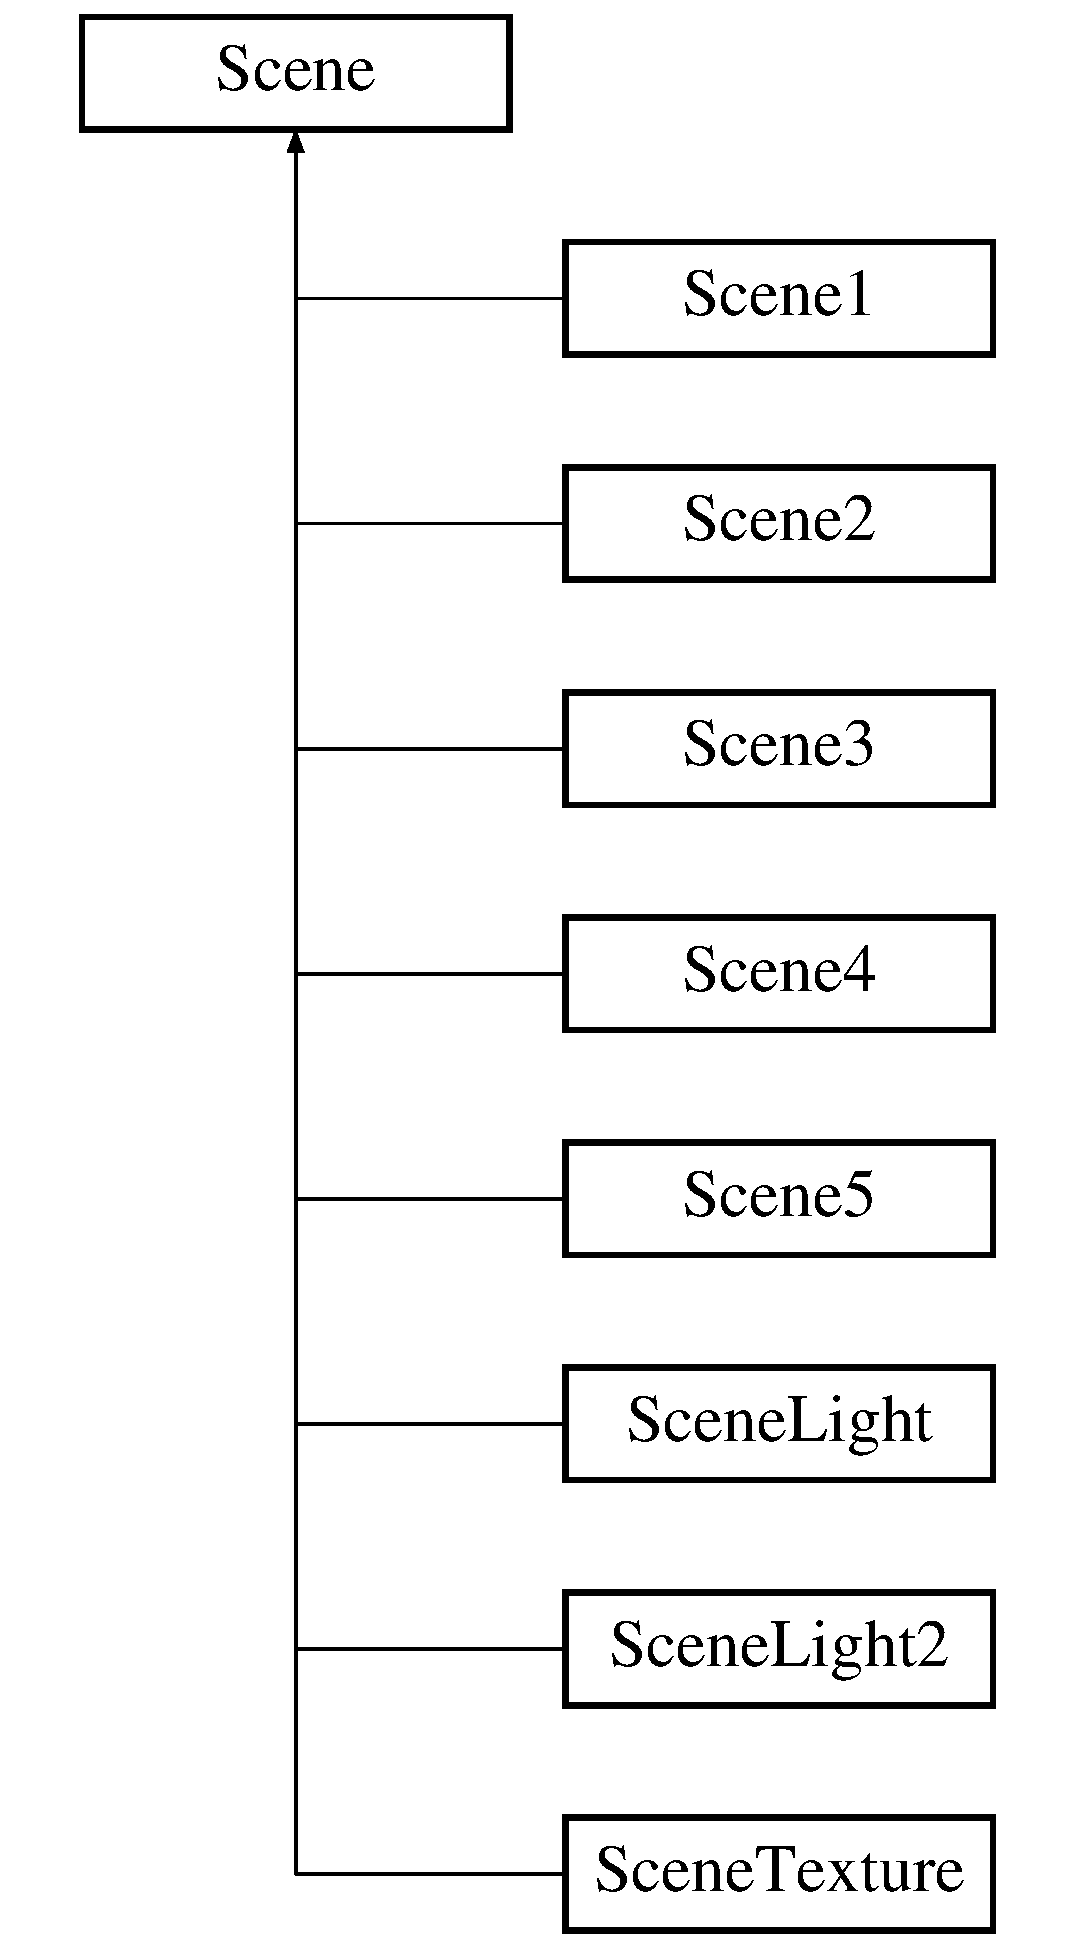
\includegraphics[height=9.000000cm]{class_scene}
\end{center}
\end{figure}
\subsection*{Public Member Functions}
\begin{DoxyCompactItemize}
\item 
\hypertarget{class_scene_ac3c4677dfd702a3ffd5ffadd3f1ac478}{virtual void {\bfseries Init} ()=0}\label{class_scene_ac3c4677dfd702a3ffd5ffadd3f1ac478}

\item 
\hypertarget{class_scene_af5c6bcf2185087fb32c27fb8f6a18d91}{virtual void {\bfseries Update} (double dt)=0}\label{class_scene_af5c6bcf2185087fb32c27fb8f6a18d91}

\item 
\hypertarget{class_scene_ae24d21e12b34839994ad265662ea24d7}{virtual void {\bfseries Render} ()=0}\label{class_scene_ae24d21e12b34839994ad265662ea24d7}

\item 
\hypertarget{class_scene_aae8e24654ef98c79961c2b804b12852c}{virtual void {\bfseries Exit} ()=0}\label{class_scene_aae8e24654ef98c79961c2b804b12852c}

\end{DoxyCompactItemize}


\subsection{Detailed Description}
Provides methods to create other \hyperlink{class_scene}{Scene} classes, it is a an abstract class by itself. 

Class \hyperlink{class_scene}{Scene}\+: 

The documentation for this class was generated from the following file\+:\begin{DoxyCompactItemize}
\item 
Scene.\+h\end{DoxyCompactItemize}

\hypertarget{class_scene1}{\section{Scene1 Class Reference}
\label{class_scene1}\index{Scene1@{Scene1}}
}
Inheritance diagram for Scene1\+:\begin{figure}[H]
\begin{center}
\leavevmode
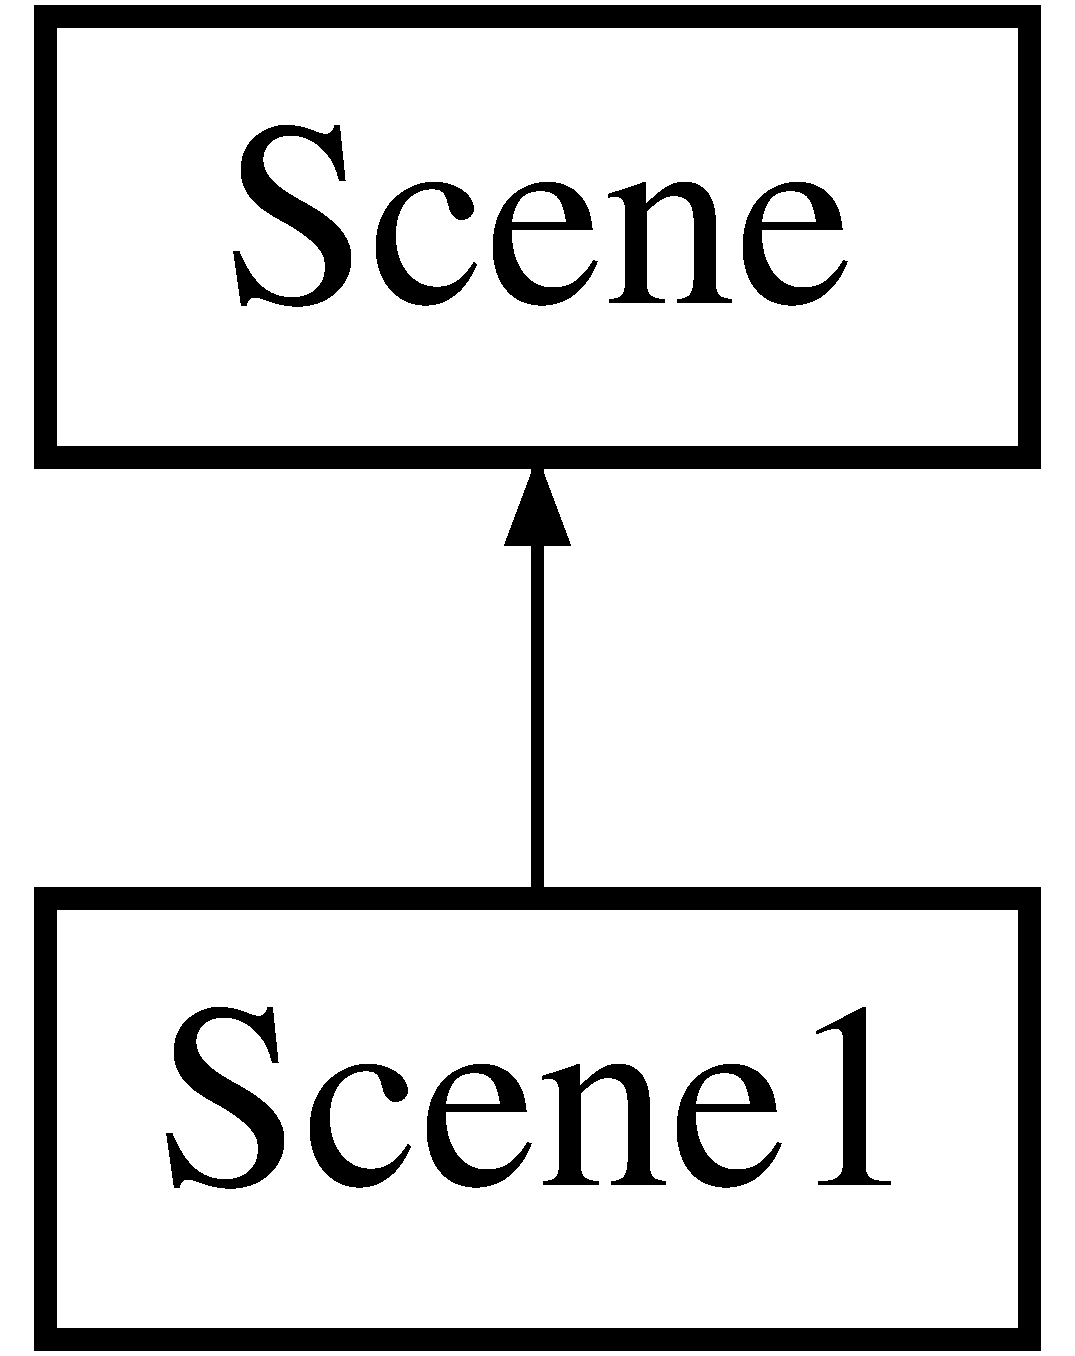
\includegraphics[height=2.000000cm]{class_scene1}
\end{center}
\end{figure}
\subsection*{Public Types}
\begin{DoxyCompactItemize}
\item 
\hypertarget{class_scene1_aa9a6ee99c64ea967c6ddc707334c89a3}{enum {\bfseries G\+E\+O\+M\+E\+T\+R\+Y\+\_\+\+T\+Y\+P\+E} \{ {\bfseries G\+E\+O\+\_\+\+T\+R\+I\+A\+N\+G\+L\+E\+\_\+1} = 0, 
{\bfseries G\+E\+O\+\_\+\+T\+R\+I\+A\+N\+G\+L\+E\+\_\+2}, 
{\bfseries N\+U\+M\+\_\+\+G\+E\+O\+M\+E\+T\+R\+Y}
 \}}\label{class_scene1_aa9a6ee99c64ea967c6ddc707334c89a3}

\end{DoxyCompactItemize}
\subsection*{Public Member Functions}
\begin{DoxyCompactItemize}
\item 
\hypertarget{class_scene1_a34e29939733a7cfe7ac71cd3110e3eb1}{virtual void {\bfseries Init} ()}\label{class_scene1_a34e29939733a7cfe7ac71cd3110e3eb1}

\item 
\hypertarget{class_scene1_a569fefef6ee64f45979ea39b8f12b2b1}{virtual void {\bfseries Update} (double dt)}\label{class_scene1_a569fefef6ee64f45979ea39b8f12b2b1}

\item 
\hypertarget{class_scene1_aa99ede8a76f1d9dac4d491c5337d559e}{virtual void {\bfseries Render} ()}\label{class_scene1_aa99ede8a76f1d9dac4d491c5337d559e}

\item 
\hypertarget{class_scene1_a61e1db3a2a15af692807f28293e98eef}{virtual void {\bfseries Exit} ()}\label{class_scene1_a61e1db3a2a15af692807f28293e98eef}

\end{DoxyCompactItemize}


The documentation for this class was generated from the following files\+:\begin{DoxyCompactItemize}
\item 
Scene1.\+h\item 
Scene1.\+cpp\end{DoxyCompactItemize}

\hypertarget{class_scene2}{\section{Scene2 Class Reference}
\label{class_scene2}\index{Scene2@{Scene2}}
}
Inheritance diagram for Scene2\+:\begin{figure}[H]
\begin{center}
\leavevmode
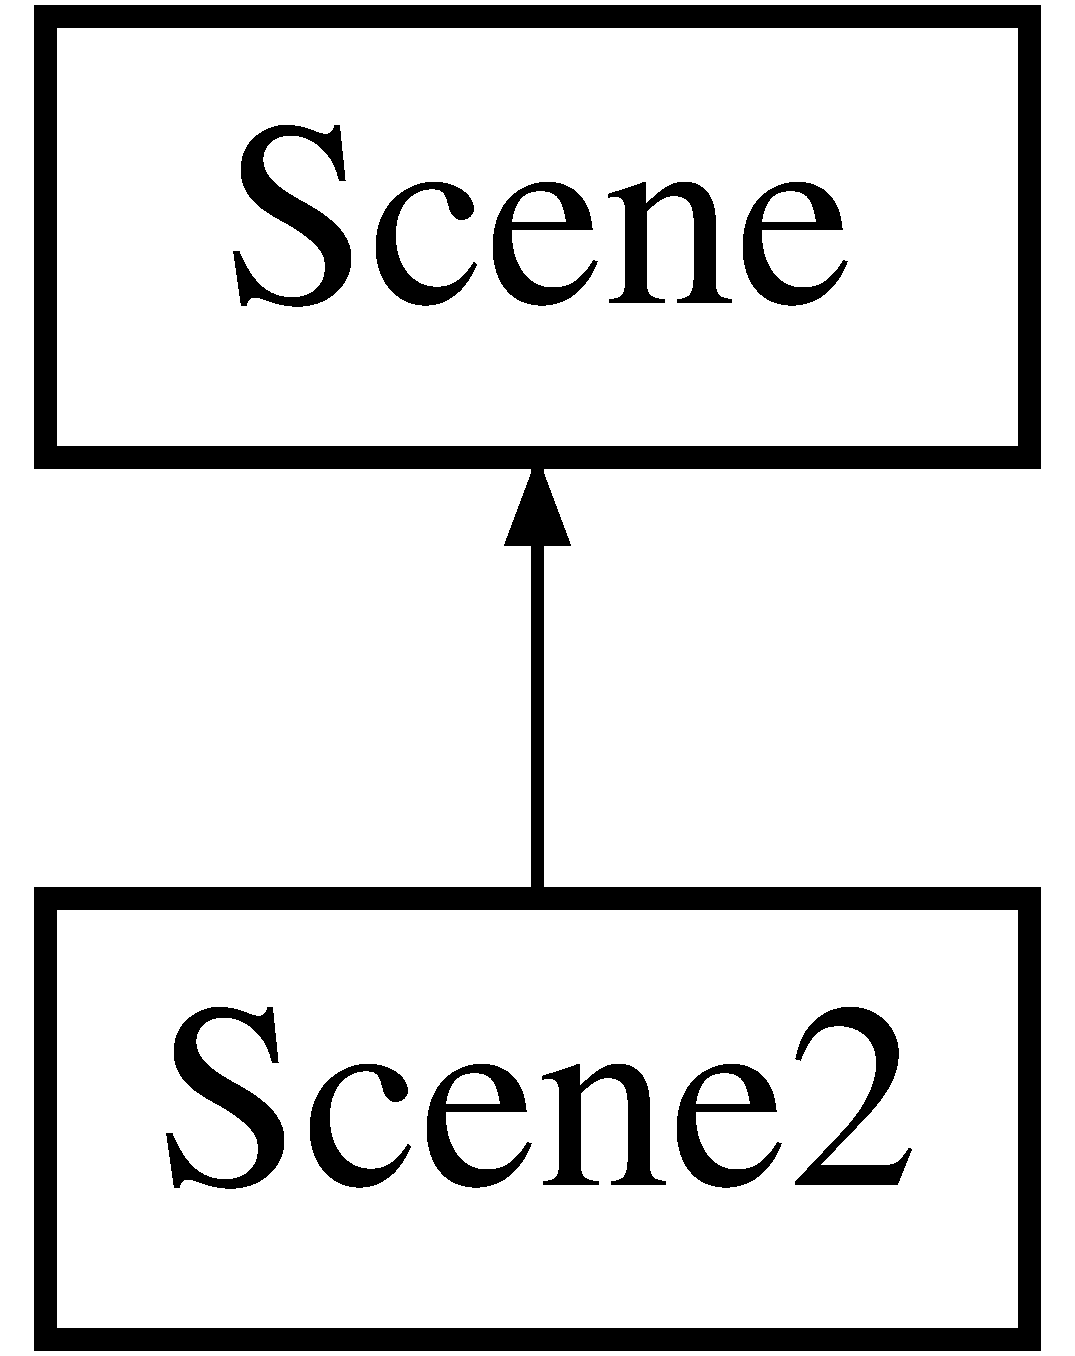
\includegraphics[height=2.000000cm]{class_scene2}
\end{center}
\end{figure}
\subsection*{Public Types}
\begin{DoxyCompactItemize}
\item 
\hypertarget{class_scene2_a028873b2024a640768bebc50fb1b0b0e}{enum {\bfseries G\+E\+O\+M\+E\+T\+R\+Y\+\_\+\+T\+Y\+P\+E} \{ \\*
{\bfseries T\+R\+I\+A\+N\+G\+L\+E} = 0, 
{\bfseries S\+T\+A\+R}, 
{\bfseries S\+Q\+U\+A\+R\+E}, 
{\bfseries O\+C\+T\+A\+G\+O\+N}, 
\\*
{\bfseries N\+U\+M\+\_\+\+G\+E\+O\+M\+E\+T\+R\+Y}
 \}}\label{class_scene2_a028873b2024a640768bebc50fb1b0b0e}

\item 
\hypertarget{class_scene2_a49448a0d6704fdddc6be96a09c943d99}{enum {\bfseries U\+N\+I\+F\+O\+R\+M\+\_\+\+T\+Y\+P\+E} \{ {\bfseries U\+\_\+\+M\+V\+P} = 0, 
{\bfseries U\+\_\+\+T\+O\+T\+A\+L}
 \}}\label{class_scene2_a49448a0d6704fdddc6be96a09c943d99}

\end{DoxyCompactItemize}
\subsection*{Public Member Functions}
\begin{DoxyCompactItemize}
\item 
\hypertarget{class_scene2_ad452e11ff007a8a1a410284630eb6f12}{virtual void {\bfseries Init} ()}\label{class_scene2_ad452e11ff007a8a1a410284630eb6f12}

\item 
\hypertarget{class_scene2_a26d9fb1c36b04d8b3dac98740f7f77e6}{virtual void {\bfseries Update} (double dt)}\label{class_scene2_a26d9fb1c36b04d8b3dac98740f7f77e6}

\item 
\hypertarget{class_scene2_ac035da5e87c59e6b1828ceec8193cea4}{virtual void {\bfseries Render} ()}\label{class_scene2_ac035da5e87c59e6b1828ceec8193cea4}

\item 
\hypertarget{class_scene2_ae4c94dab85cfe1e734af4e288060dec4}{virtual void {\bfseries Exit} ()}\label{class_scene2_ae4c94dab85cfe1e734af4e288060dec4}

\end{DoxyCompactItemize}
\subsection*{Public Attributes}
\begin{DoxyCompactItemize}
\item 
\hypertarget{class_scene2_a91fa51259776242875a07ed6dba78bd0}{unsigned {\bfseries m\+\_\+parameters} \mbox{[}U\+\_\+\+T\+O\+T\+A\+L\mbox{]}}\label{class_scene2_a91fa51259776242875a07ed6dba78bd0}

\item 
\hypertarget{class_scene2_af1e450d21db6d3ea63232aea222681df}{float {\bfseries rotate\+Angle}}\label{class_scene2_af1e450d21db6d3ea63232aea222681df}

\item 
\hypertarget{class_scene2_a08edb88515cde967432df36ade24bc6f}{float {\bfseries translate\+X}}\label{class_scene2_a08edb88515cde967432df36ade24bc6f}

\item 
\hypertarget{class_scene2_a26b9f96854b0b2ae955b2d85dccf0341}{float {\bfseries scale\+All}}\label{class_scene2_a26b9f96854b0b2ae955b2d85dccf0341}

\item 
\hypertarget{class_scene2_a924b2a2e5ac0c951dea8bec7b52f6f2e}{float {\bfseries rotate\+Angle2}}\label{class_scene2_a924b2a2e5ac0c951dea8bec7b52f6f2e}

\item 
\hypertarget{class_scene2_ace313221ca13f71cb90ff42006ff9051}{float {\bfseries randomiser}}\label{class_scene2_ace313221ca13f71cb90ff42006ff9051}

\end{DoxyCompactItemize}


The documentation for this class was generated from the following files\+:\begin{DoxyCompactItemize}
\item 
Scene2.\+h\item 
Scene2.\+cpp\end{DoxyCompactItemize}

\hypertarget{class_scene3}{\section{Scene3 Class Reference}
\label{class_scene3}\index{Scene3@{Scene3}}
}
Inheritance diagram for Scene3\+:\begin{figure}[H]
\begin{center}
\leavevmode
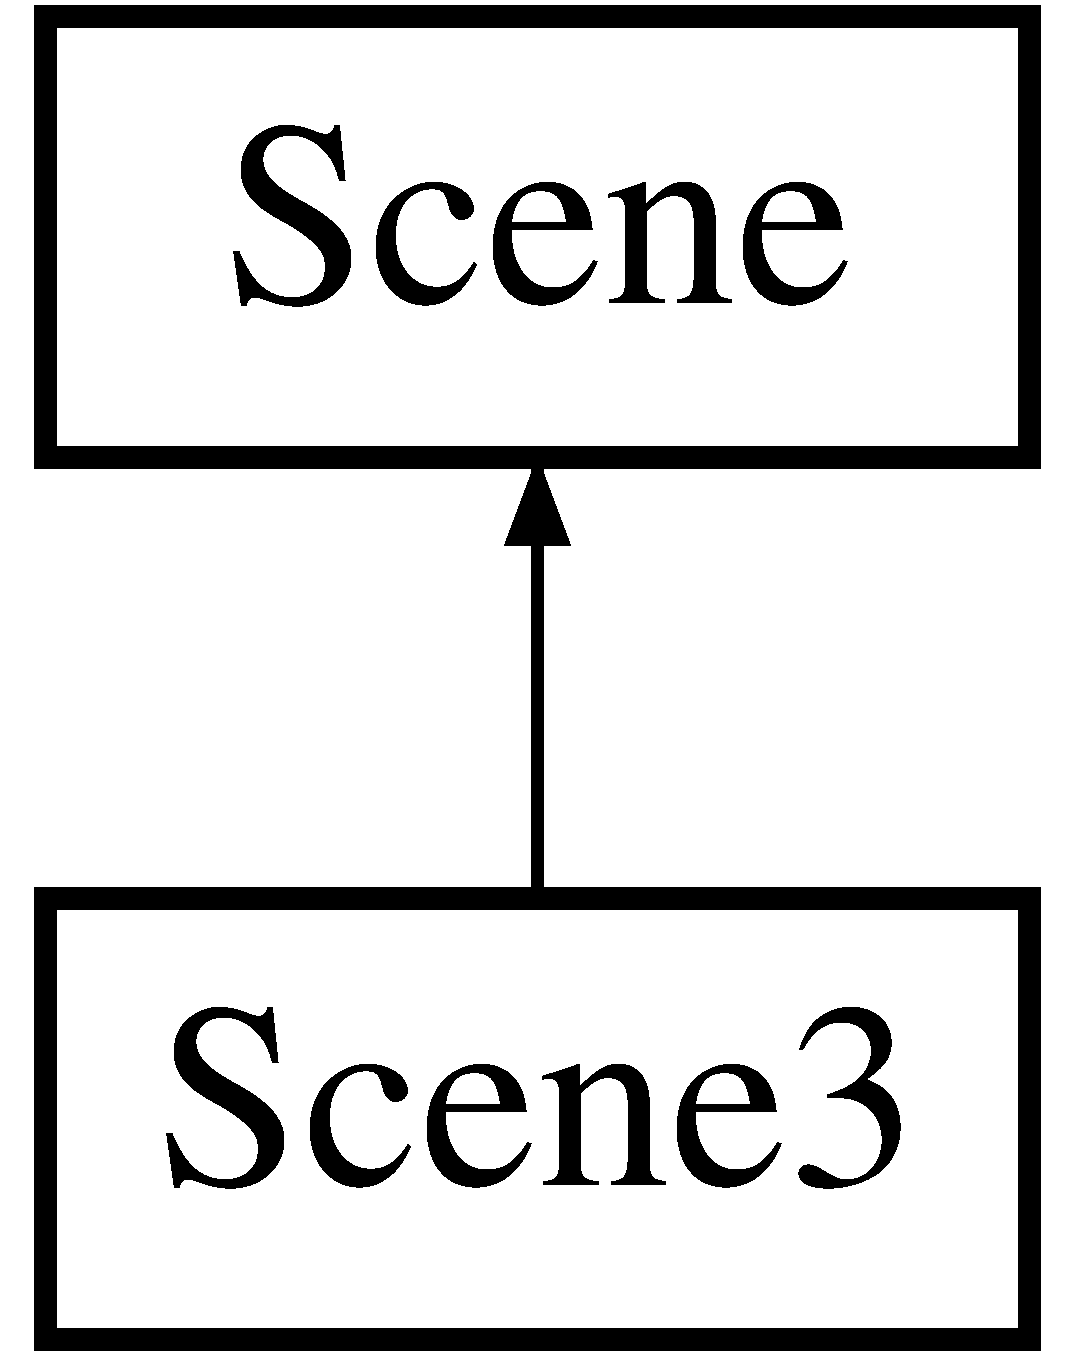
\includegraphics[height=2.000000cm]{class_scene3}
\end{center}
\end{figure}
\subsection*{Public Member Functions}
\begin{DoxyCompactItemize}
\item 
\hypertarget{class_scene3_ae0fa7e48f701d3761d8c6ca01a334feb}{virtual void {\bfseries Init} ()}\label{class_scene3_ae0fa7e48f701d3761d8c6ca01a334feb}

\item 
\hypertarget{class_scene3_ac6aee0665d9f41f4a009fdcb29ac40f1}{virtual void {\bfseries Update} (double dt)}\label{class_scene3_ac6aee0665d9f41f4a009fdcb29ac40f1}

\item 
\hypertarget{class_scene3_aca22983af978d16e380bf5ca4ceab143}{virtual void {\bfseries Render} ()}\label{class_scene3_aca22983af978d16e380bf5ca4ceab143}

\item 
\hypertarget{class_scene3_a71f49cdf7e105d554c2c8f03b720cdc9}{virtual void {\bfseries Exit} ()}\label{class_scene3_a71f49cdf7e105d554c2c8f03b720cdc9}

\end{DoxyCompactItemize}


The documentation for this class was generated from the following files\+:\begin{DoxyCompactItemize}
\item 
Scene3.\+h\item 
Scene3.\+cpp\end{DoxyCompactItemize}

\hypertarget{class_scene4}{\section{Scene4 Class Reference}
\label{class_scene4}\index{Scene4@{Scene4}}
}
Inheritance diagram for Scene4\+:\begin{figure}[H]
\begin{center}
\leavevmode
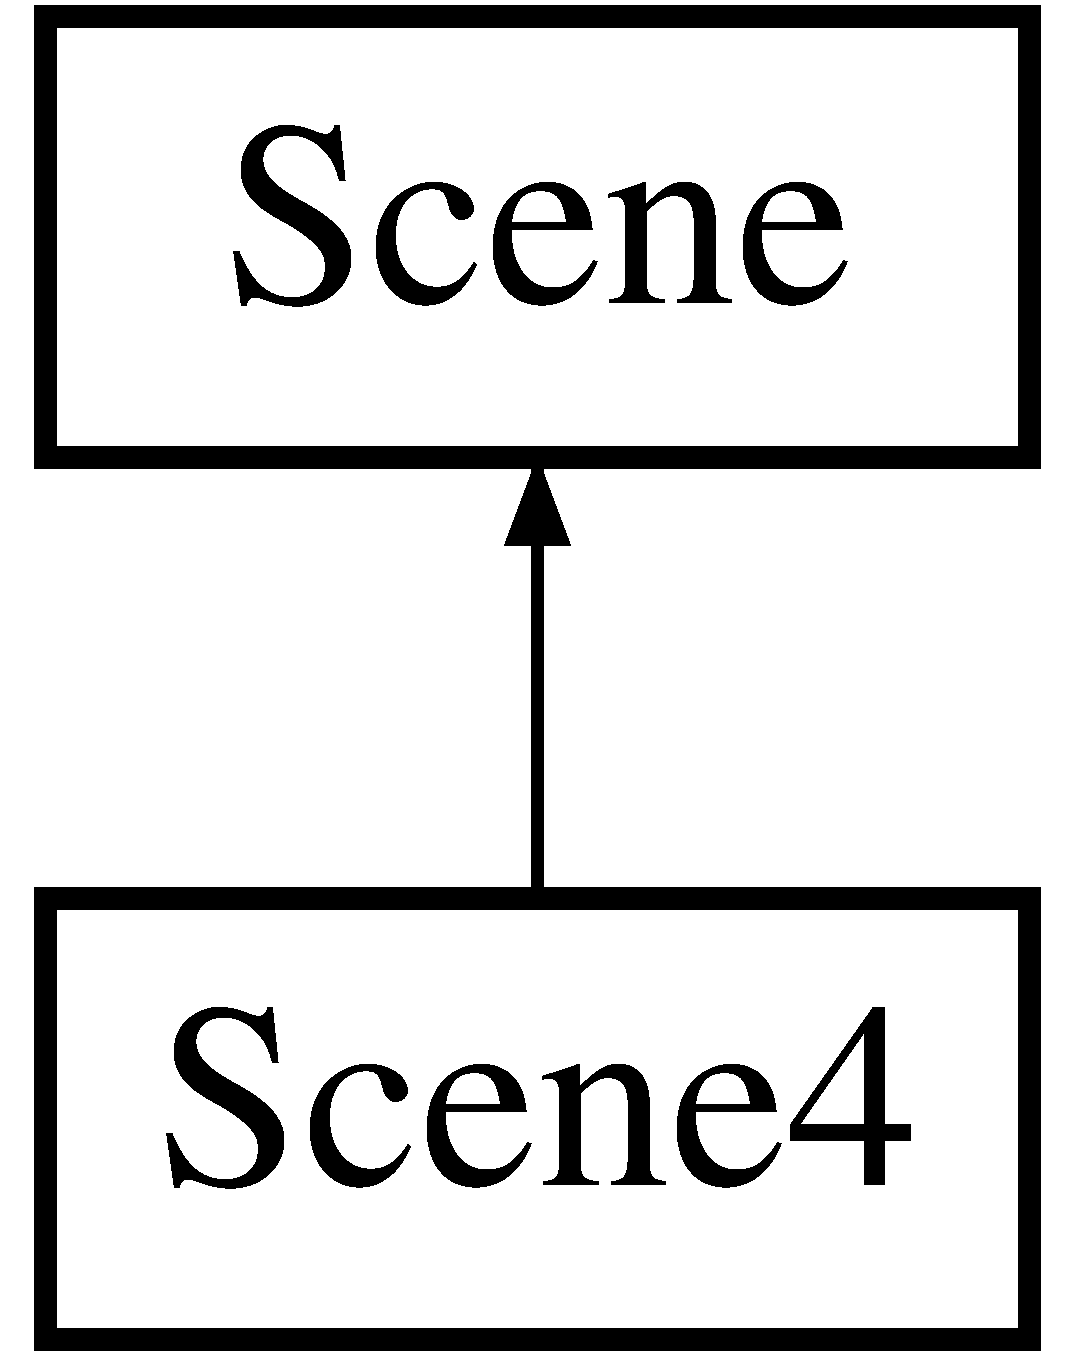
\includegraphics[height=2.000000cm]{class_scene4}
\end{center}
\end{figure}
\subsection*{Public Member Functions}
\begin{DoxyCompactItemize}
\item 
\hypertarget{class_scene4_a3df44b08162c976706aa49ceef9e9f1a}{virtual void {\bfseries Init} ()}\label{class_scene4_a3df44b08162c976706aa49ceef9e9f1a}

\item 
\hypertarget{class_scene4_abfad5f484a4cc6e8a4b58c149e9ade21}{virtual void {\bfseries Update} (double dt)}\label{class_scene4_abfad5f484a4cc6e8a4b58c149e9ade21}

\item 
\hypertarget{class_scene4_aedb8a31e5bde1b6ad9d8127a0ac393da}{virtual void {\bfseries Render} ()}\label{class_scene4_aedb8a31e5bde1b6ad9d8127a0ac393da}

\item 
\hypertarget{class_scene4_a06cde399a3cda7d85d69773eb16237a9}{virtual void {\bfseries Exit} ()}\label{class_scene4_a06cde399a3cda7d85d69773eb16237a9}

\end{DoxyCompactItemize}


The documentation for this class was generated from the following files\+:\begin{DoxyCompactItemize}
\item 
Scene4.\+h\item 
Scene4.\+cpp\end{DoxyCompactItemize}

\hypertarget{class_scene5}{\section{Scene5 Class Reference}
\label{class_scene5}\index{Scene5@{Scene5}}
}
Inheritance diagram for Scene5\+:\begin{figure}[H]
\begin{center}
\leavevmode
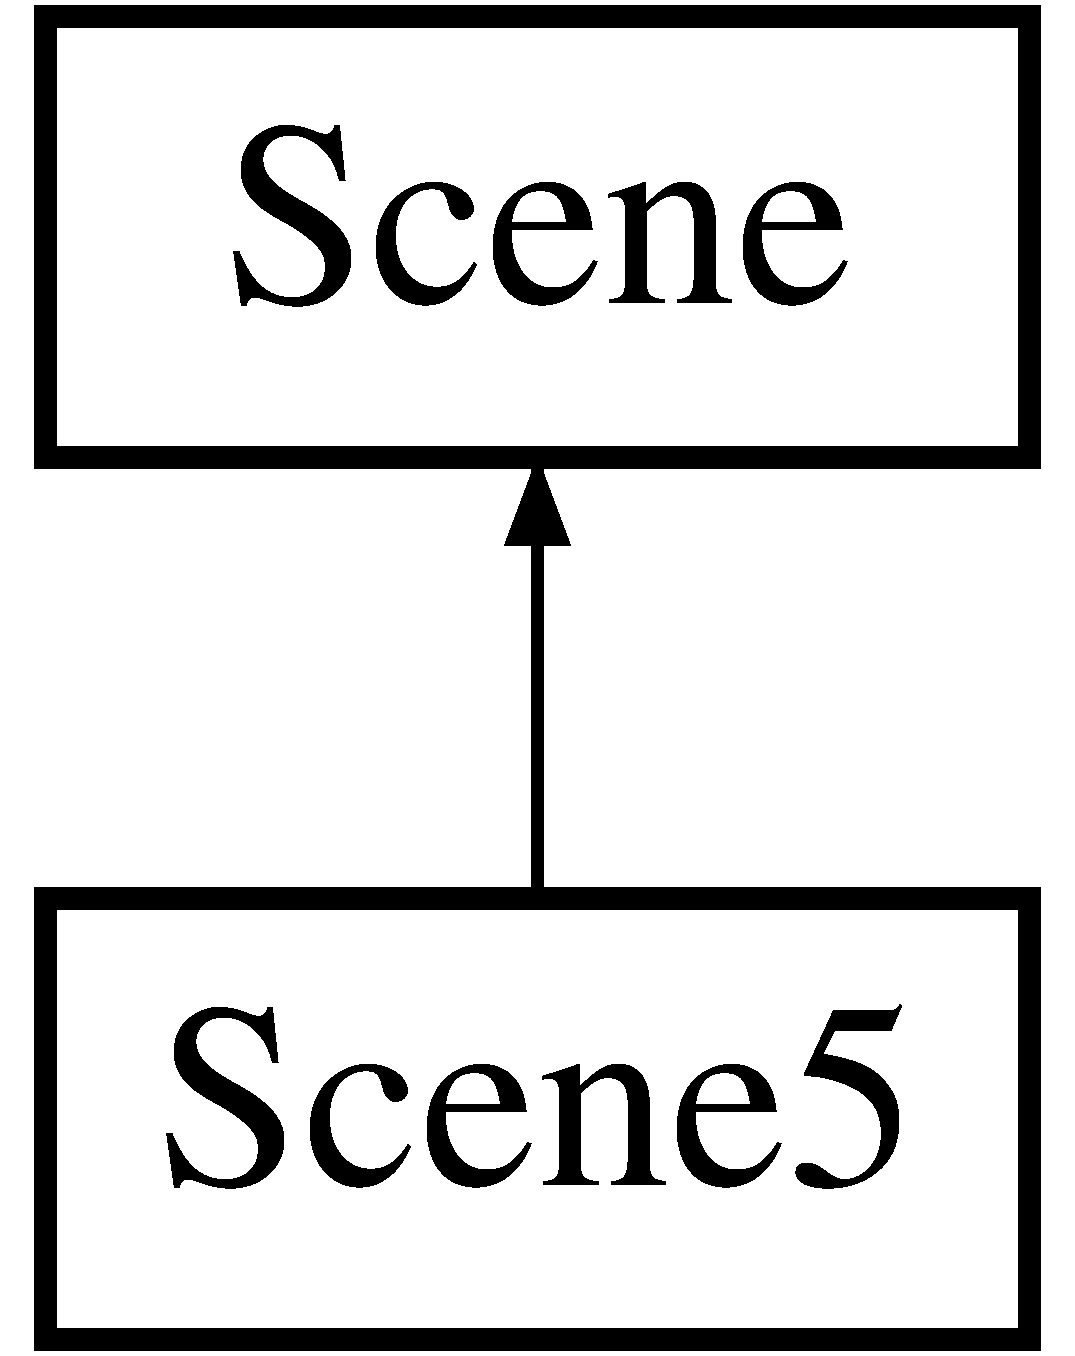
\includegraphics[height=2.000000cm]{class_scene5}
\end{center}
\end{figure}
\subsection*{Public Member Functions}
\begin{DoxyCompactItemize}
\item 
\hypertarget{class_scene5_a3005bc4ce693f3bd956e2e5bc0a3e2eb}{virtual void {\bfseries Init} ()}\label{class_scene5_a3005bc4ce693f3bd956e2e5bc0a3e2eb}

\item 
\hypertarget{class_scene5_aed582dc4f5c2fee3d6f8937a51bf496d}{virtual void {\bfseries Update} (double dt)}\label{class_scene5_aed582dc4f5c2fee3d6f8937a51bf496d}

\item 
\hypertarget{class_scene5_af3869e6d4fd6c1be91e20642ae41f5a5}{virtual void {\bfseries Render} ()}\label{class_scene5_af3869e6d4fd6c1be91e20642ae41f5a5}

\item 
\hypertarget{class_scene5_a093e65758de039397dcb876a78fa199c}{virtual void {\bfseries Exit} ()}\label{class_scene5_a093e65758de039397dcb876a78fa199c}

\end{DoxyCompactItemize}


The documentation for this class was generated from the following files\+:\begin{DoxyCompactItemize}
\item 
Scene5.\+h\item 
Scene5.\+cpp\end{DoxyCompactItemize}

\hypertarget{class_scene_light}{\section{Scene\+Light Class Reference}
\label{class_scene_light}\index{Scene\+Light@{Scene\+Light}}
}


Provides methods to create variables and functions to use for modelling.  




{\ttfamily \#include $<$Scene\+Light.\+h$>$}

Inheritance diagram for Scene\+Light\+:\begin{figure}[H]
\begin{center}
\leavevmode
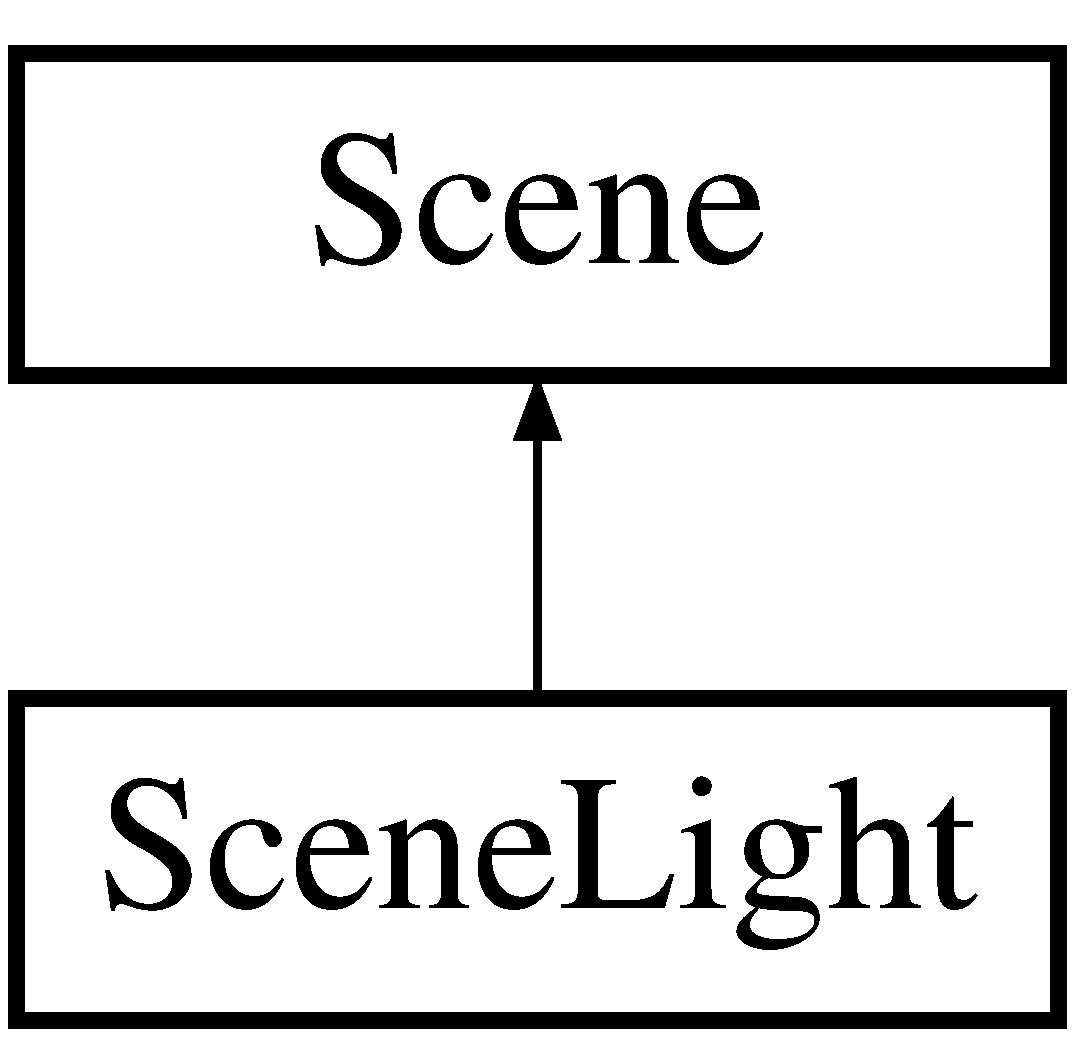
\includegraphics[height=2.000000cm]{class_scene_light}
\end{center}
\end{figure}
\subsection*{Public Member Functions}
\begin{DoxyCompactItemize}
\item 
\hypertarget{class_scene_light_a9efc7124efacb45a7cce730688bf20e9}{virtual void {\bfseries Init} ()}\label{class_scene_light_a9efc7124efacb45a7cce730688bf20e9}

\item 
virtual void \hyperlink{class_scene_light_a23681b3a667399752645d5763ddc72a7}{Update} (double dt)
\item 
\hypertarget{class_scene_light_a9088eb7ba6a1d55ebe9e0094c67281bf}{virtual void {\bfseries Render} ()}\label{class_scene_light_a9088eb7ba6a1d55ebe9e0094c67281bf}

\item 
\hypertarget{class_scene_light_afe406a984481b2bc235c445beb2165f9}{virtual void {\bfseries Exit} ()}\label{class_scene_light_afe406a984481b2bc235c445beb2165f9}

\item 
\hypertarget{class_scene_light_a308b74cd5d6e958ca12bd698e2dcd2b8}{void {\bfseries Render\+Body} ()}\label{class_scene_light_a308b74cd5d6e958ca12bd698e2dcd2b8}

\item 
\hypertarget{class_scene_light_aa125d25f061fc64d484d7f18266f0aaa}{void {\bfseries Render\+Limb} ()}\label{class_scene_light_aa125d25f061fc64d484d7f18266f0aaa}

\item 
\hypertarget{class_scene_light_a9da10b516c791c3a2cf5c2faec7f38bc}{void {\bfseries Render\+Robot} ()}\label{class_scene_light_a9da10b516c791c3a2cf5c2faec7f38bc}

\item 
void \hyperlink{class_scene_light_aee8ec7a58c9f640e37868992f497d0ce}{Pikachu\+Left\+Ears} ()
\begin{DoxyCompactList}\small\item\em Pikachu\+Left\+Ears nad Pikachu\+Right\+Ears are both functions used to create the ears of Pikachu and then it will be called in Pikachu\+Head. \end{DoxyCompactList}\item 
\hypertarget{class_scene_light_ae877dac3bd1285d70c45a715ea952dfe}{void {\bfseries Pikachu\+Right\+Ears} ()}\label{class_scene_light_ae877dac3bd1285d70c45a715ea952dfe}

\item 
void \hyperlink{class_scene_light_ad60deb62dc3a5570e8c9c4c809951df6}{Pikachu\+Head} ()
\begin{DoxyCompactList}\small\item\em Pikachu\+Head is a fucntion call where i combine all the parts of Pikachu's head in a single function call. \end{DoxyCompactList}\item 
void \hyperlink{class_scene_light_a6ed17a486082d6fa33480124e0c3c6fe}{Pikachu\+Eyes} ()
\begin{DoxyCompactList}\small\item\em Pikachu\+Eyes is a function used to create the eyes of Pikachu and then it will be called in Pikachu\+Head. \end{DoxyCompactList}\item 
void \hyperlink{class_scene_light_a2dac04dba19c6c12dfd1917395cf567b}{Pikachu\+Nose} ()
\begin{DoxyCompactList}\small\item\em Pikachu\+Nose and Pikachu Mouth are both function used to create the nose and mouth of Pikachu respectively and then it will be called in Pikachu\+Head. \end{DoxyCompactList}\item 
\hypertarget{class_scene_light_a21975d512f03405c6f4cc5ffb4e04300}{void {\bfseries Pikachu\+Mouth} ()}\label{class_scene_light_a21975d512f03405c6f4cc5ffb4e04300}

\item 
void \hyperlink{class_scene_light_a4b3aadf3c9ad220a1cd19e39480c7956}{Pikachu\+Body} ()
\begin{DoxyCompactList}\small\item\em Pikachu\+Body is a function used to create the body of Pikachu and then it will be called in Render\+Pikachu. \end{DoxyCompactList}\item 
void \hyperlink{class_scene_light_a3a0513d87de1bdc3a750b85524655bb9}{Pikachu\+Left\+Hands} ()
\begin{DoxyCompactList}\small\item\em Pikachu\+Left\+Hands and Pikachu\+Right\+Hands are both function used to create the hands of pikachu respectively before being callled in Render\+Pikachu. \end{DoxyCompactList}\item 
\hypertarget{class_scene_light_a82e9b15e5dfc4bd07ab1c73e1824cf04}{void {\bfseries Pikachu\+Right\+Hands} ()}\label{class_scene_light_a82e9b15e5dfc4bd07ab1c73e1824cf04}

\item 
void \hyperlink{class_scene_light_a51d4b22f8c6bf6d74225fd1725181603}{Pikachu\+Left\+Feet} ()
\begin{DoxyCompactList}\small\item\em Pikachu\+Left\+Feet and Pikachu\+Right\+Feet are both function used to create the feet of pikachu respectively before being callled in Render\+Pikachu. \end{DoxyCompactList}\item 
\hypertarget{class_scene_light_a5272028872a63074703f6b7470162d63}{void {\bfseries Pikachu\+Right\+Feet} ()}\label{class_scene_light_a5272028872a63074703f6b7470162d63}

\item 
void \hyperlink{class_scene_light_a8a23c6a2b293b2b8f81a5846865d34d1}{Pikachu\+Backstrip} ()
\begin{DoxyCompactList}\small\item\em Pikachu\+Backstrip is a function used to create the back strip of pikachu before being callled in Render\+Pikachu. \end{DoxyCompactList}\item 
void \hyperlink{class_scene_light_aad5eca9ad5ec115755aff98227547df3}{Pikachu\+Tail} ()
\begin{DoxyCompactList}\small\item\em Pikachu\+Tail is a function used to create the tail of pikachu before being callled in Render\+Pikachu. \end{DoxyCompactList}\item 
void \hyperlink{class_scene_light_aec85835deabe218d774b397ce8a1c18e}{Render\+Pikachu} ()
\begin{DoxyCompactList}\small\item\em Render\+Pikachu is a function used to accomdate all the other Pikachu's parts that i have created before it it called in render so as to keep the code clean. \end{DoxyCompactList}\item 
void \hyperlink{class_scene_light_adb3c2941d33259cf9ba58f9e2d6fb96f}{Poke\+Ball\+Top} ()
\begin{DoxyCompactList}\small\item\em Poke\+Ball\+Top is a function used to create the top part of the pokeball. \end{DoxyCompactList}\item 
void \hyperlink{class_scene_light_a35bb7ede9ffd535ca637a521ce472a16}{Pokeball\+Bottom} ()
\begin{DoxyCompactList}\small\item\em Pokeball\+Bottom is a function used to create the bottom part of the pokeball. \end{DoxyCompactList}\item 
void \hyperlink{class_scene_light_a3e2e9d713c572bd248ebfa3bfa176004}{Render\+Pokeball} ()
\begin{DoxyCompactList}\small\item\em Render\+Pokeball is a function used to accomdate all the other Pokeball's parts that i have created before it it called in render so as to keep the code clean. \end{DoxyCompactList}\item 
\hypertarget{class_scene_light_ab21debc8928012f3f824df19aa7a2c35}{void {\bfseries debug\+Print} ()}\label{class_scene_light_ab21debc8928012f3f824df19aa7a2c35}

\end{DoxyCompactItemize}


\subsection{Detailed Description}
Provides methods to create variables and functions to use for modelling. 

Class \hyperlink{class_scene_light}{Scene\+Light}\+: 

\subsection{Member Function Documentation}
\hypertarget{class_scene_light_a8a23c6a2b293b2b8f81a5846865d34d1}{\index{Scene\+Light@{Scene\+Light}!Pikachu\+Backstrip@{Pikachu\+Backstrip}}
\index{Pikachu\+Backstrip@{Pikachu\+Backstrip}!Scene\+Light@{Scene\+Light}}
\subsubsection[{Pikachu\+Backstrip}]{\setlength{\rightskip}{0pt plus 5cm}void Scene\+Light\+::\+Pikachu\+Backstrip (
\begin{DoxyParamCaption}
{}
\end{DoxyParamCaption}
)}}\label{class_scene_light_a8a23c6a2b293b2b8f81a5846865d34d1}


Pikachu\+Backstrip is a function used to create the back strip of pikachu before being callled in Render\+Pikachu. 


\begin{DoxyParams}{Parameters}
{\em 2} & Sphere scaled Shpaes Variable\+: G\+E\+O\+\_\+\+B\+A\+C\+K\+S\+T\+R\+I\+P \\
\hline
\end{DoxyParams}
\hypertarget{class_scene_light_a4b3aadf3c9ad220a1cd19e39480c7956}{\index{Scene\+Light@{Scene\+Light}!Pikachu\+Body@{Pikachu\+Body}}
\index{Pikachu\+Body@{Pikachu\+Body}!Scene\+Light@{Scene\+Light}}
\subsubsection[{Pikachu\+Body}]{\setlength{\rightskip}{0pt plus 5cm}void Scene\+Light\+::\+Pikachu\+Body (
\begin{DoxyParamCaption}
{}
\end{DoxyParamCaption}
)}}\label{class_scene_light_a4b3aadf3c9ad220a1cd19e39480c7956}


Pikachu\+Body is a function used to create the body of Pikachu and then it will be called in Render\+Pikachu. 


\begin{DoxyParams}{Parameters}
{\em 2} & Hemi\+Sphere Shpaes Variable\+: G\+E\+O\+\_\+\+P\+I\+K\+A\+C\+H\+U\+H\+E\+A\+D\+P\+A\+R\+T\+S \\
\hline
\end{DoxyParams}
\hypertarget{class_scene_light_a6ed17a486082d6fa33480124e0c3c6fe}{\index{Scene\+Light@{Scene\+Light}!Pikachu\+Eyes@{Pikachu\+Eyes}}
\index{Pikachu\+Eyes@{Pikachu\+Eyes}!Scene\+Light@{Scene\+Light}}
\subsubsection[{Pikachu\+Eyes}]{\setlength{\rightskip}{0pt plus 5cm}void Scene\+Light\+::\+Pikachu\+Eyes (
\begin{DoxyParamCaption}
{}
\end{DoxyParamCaption}
)}}\label{class_scene_light_a6ed17a486082d6fa33480124e0c3c6fe}


Pikachu\+Eyes is a function used to create the eyes of Pikachu and then it will be called in Pikachu\+Head. 


\begin{DoxyParams}{Parameters}
{\em 2} & Sphere scaled to near flat shape Shape Variable\+: G\+E\+O\+\_\+\+P\+I\+K\+A\+C\+H\+U\+E\+Y\+E\+S and G\+O\+E\+\_\+\+P\+I\+K\+A\+C\+H\+U\+E\+Y\+E\+S\+W\+H\+I\+T\+E \\
\hline
\end{DoxyParams}
\hypertarget{class_scene_light_ad60deb62dc3a5570e8c9c4c809951df6}{\index{Scene\+Light@{Scene\+Light}!Pikachu\+Head@{Pikachu\+Head}}
\index{Pikachu\+Head@{Pikachu\+Head}!Scene\+Light@{Scene\+Light}}
\subsubsection[{Pikachu\+Head}]{\setlength{\rightskip}{0pt plus 5cm}void Scene\+Light\+::\+Pikachu\+Head (
\begin{DoxyParamCaption}
{}
\end{DoxyParamCaption}
)}}\label{class_scene_light_ad60deb62dc3a5570e8c9c4c809951df6}


Pikachu\+Head is a fucntion call where i combine all the parts of Pikachu's head in a single function call. 


\begin{DoxyParams}{Parameters}
{\em Shape} & Variable\+: G\+E\+O\+\_\+\+P\+I\+K\+A\+C\+H\+U\+H\+E\+A\+D\+P\+A\+R\+T\+S, G\+E\+O\+\_\+\+P\+I\+K\+A\+C\+H\+U\+H\+E\+A\+D\+P\+A\+R\+T\+S3 Function called\+: Pikachu\+Right\+Ears, Pikachu\+Left\+Ears, Pikachu\+Eyes, Pikachu\+Month, Pikachu\+Nose \\
\hline
\end{DoxyParams}
\hypertarget{class_scene_light_aee8ec7a58c9f640e37868992f497d0ce}{\index{Scene\+Light@{Scene\+Light}!Pikachu\+Left\+Ears@{Pikachu\+Left\+Ears}}
\index{Pikachu\+Left\+Ears@{Pikachu\+Left\+Ears}!Scene\+Light@{Scene\+Light}}
\subsubsection[{Pikachu\+Left\+Ears}]{\setlength{\rightskip}{0pt plus 5cm}void Scene\+Light\+::\+Pikachu\+Left\+Ears (
\begin{DoxyParamCaption}
{}
\end{DoxyParamCaption}
)}}\label{class_scene_light_aee8ec7a58c9f640e37868992f497d0ce}


Pikachu\+Left\+Ears nad Pikachu\+Right\+Ears are both functions used to create the ears of Pikachu and then it will be called in Pikachu\+Head. 


\begin{DoxyParams}{Parameters}
{\em 2} & Cone for each function Total 4 cones Shape Variable\+: G\+E\+O\+\_\+\+C\+O\+N\+E\+Yellow and G\+E\+O\+\_\+\+C\+O\+N\+E\+Black \\
\hline
\end{DoxyParams}
\hypertarget{class_scene_light_a51d4b22f8c6bf6d74225fd1725181603}{\index{Scene\+Light@{Scene\+Light}!Pikachu\+Left\+Feet@{Pikachu\+Left\+Feet}}
\index{Pikachu\+Left\+Feet@{Pikachu\+Left\+Feet}!Scene\+Light@{Scene\+Light}}
\subsubsection[{Pikachu\+Left\+Feet}]{\setlength{\rightskip}{0pt plus 5cm}void Scene\+Light\+::\+Pikachu\+Left\+Feet (
\begin{DoxyParamCaption}
{}
\end{DoxyParamCaption}
)}}\label{class_scene_light_a51d4b22f8c6bf6d74225fd1725181603}


Pikachu\+Left\+Feet and Pikachu\+Right\+Feet are both function used to create the feet of pikachu respectively before being callled in Render\+Pikachu. 


\begin{DoxyParams}{Parameters}
{\em 1} & Sphere scaled 3 Hemisphere scaled for the lines Shpaes Variable\+: G\+E\+O\+\_\+\+S\+P\+H\+E\+R\+E, G\+E\+O\+\_\+\+P\+I\+K\+A\+C\+H\+U\+E\+Y\+E\+S \\
\hline
\end{DoxyParams}
\hypertarget{class_scene_light_a3a0513d87de1bdc3a750b85524655bb9}{\index{Scene\+Light@{Scene\+Light}!Pikachu\+Left\+Hands@{Pikachu\+Left\+Hands}}
\index{Pikachu\+Left\+Hands@{Pikachu\+Left\+Hands}!Scene\+Light@{Scene\+Light}}
\subsubsection[{Pikachu\+Left\+Hands}]{\setlength{\rightskip}{0pt plus 5cm}void Scene\+Light\+::\+Pikachu\+Left\+Hands (
\begin{DoxyParamCaption}
{}
\end{DoxyParamCaption}
)}}\label{class_scene_light_a3a0513d87de1bdc3a750b85524655bb9}


Pikachu\+Left\+Hands and Pikachu\+Right\+Hands are both function used to create the hands of pikachu respectively before being callled in Render\+Pikachu. 


\begin{DoxyParams}{Parameters}
{\em 1} & Sphere scaled 3 Hemisphere scaled for the lines Shpaes Variable\+: G\+E\+O\+\_\+\+S\+P\+H\+E\+R\+E, G\+E\+O\+\_\+\+P\+I\+K\+A\+C\+H\+U\+E\+Y\+E\+S \\
\hline
\end{DoxyParams}
\hypertarget{class_scene_light_a2dac04dba19c6c12dfd1917395cf567b}{\index{Scene\+Light@{Scene\+Light}!Pikachu\+Nose@{Pikachu\+Nose}}
\index{Pikachu\+Nose@{Pikachu\+Nose}!Scene\+Light@{Scene\+Light}}
\subsubsection[{Pikachu\+Nose}]{\setlength{\rightskip}{0pt plus 5cm}void Scene\+Light\+::\+Pikachu\+Nose (
\begin{DoxyParamCaption}
{}
\end{DoxyParamCaption}
)}}\label{class_scene_light_a2dac04dba19c6c12dfd1917395cf567b}


Pikachu\+Nose and Pikachu Mouth are both function used to create the nose and mouth of Pikachu respectively and then it will be called in Pikachu\+Head. 


\begin{DoxyParams}{Parameters}
{\em 2} & Hemi\+Sphere scaled differently Shape Variable\+: G\+E\+O\+\_\+\+P\+I\+K\+A\+C\+H\+U\+N\+O\+S\+E and G\+E\+O\+\_\+\+P\+I\+K\+A\+C\+H\+U\+B\+R\+O\+W\+N \\
\hline
\end{DoxyParams}
\hypertarget{class_scene_light_aad5eca9ad5ec115755aff98227547df3}{\index{Scene\+Light@{Scene\+Light}!Pikachu\+Tail@{Pikachu\+Tail}}
\index{Pikachu\+Tail@{Pikachu\+Tail}!Scene\+Light@{Scene\+Light}}
\subsubsection[{Pikachu\+Tail}]{\setlength{\rightskip}{0pt plus 5cm}void Scene\+Light\+::\+Pikachu\+Tail (
\begin{DoxyParamCaption}
{}
\end{DoxyParamCaption}
)}}\label{class_scene_light_aad5eca9ad5ec115755aff98227547df3}


Pikachu\+Tail is a function used to create the tail of pikachu before being callled in Render\+Pikachu. 


\begin{DoxyParams}{Parameters}
{\em 12} & Triangles 5 Squares Shpaes Variable\+: G\+E\+O\+\_\+\+C\+U\+B\+E, G\+E\+O\+\_\+\+T\+A\+I\+L\+Y\+E\+L\+L\+O\+W, G\+E\+O\+\_\+\+T\+A\+I\+L\+B\+R\+O\+W\+N \\
\hline
\end{DoxyParams}
\hypertarget{class_scene_light_a35bb7ede9ffd535ca637a521ce472a16}{\index{Scene\+Light@{Scene\+Light}!Pokeball\+Bottom@{Pokeball\+Bottom}}
\index{Pokeball\+Bottom@{Pokeball\+Bottom}!Scene\+Light@{Scene\+Light}}
\subsubsection[{Pokeball\+Bottom}]{\setlength{\rightskip}{0pt plus 5cm}void Scene\+Light\+::\+Pokeball\+Bottom (
\begin{DoxyParamCaption}
{}
\end{DoxyParamCaption}
)}}\label{class_scene_light_a35bb7ede9ffd535ca637a521ce472a16}


Pokeball\+Bottom is a function used to create the bottom part of the pokeball. 


\begin{DoxyParams}{Parameters}
{\em Shapes} & Variable\+: G\+E\+O\+\_\+\+P\+O\+K\+E\+B\+A\+L\+L\+W\+H\+I\+T\+E2 and G\+E\+O\+\_\+\+P\+O\+K\+E\+B\+A\+L\+L\+B\+L\+A\+C\+K \\
\hline
\end{DoxyParams}
\hypertarget{class_scene_light_adb3c2941d33259cf9ba58f9e2d6fb96f}{\index{Scene\+Light@{Scene\+Light}!Poke\+Ball\+Top@{Poke\+Ball\+Top}}
\index{Poke\+Ball\+Top@{Poke\+Ball\+Top}!Scene\+Light@{Scene\+Light}}
\subsubsection[{Poke\+Ball\+Top}]{\setlength{\rightskip}{0pt plus 5cm}void Scene\+Light\+::\+Poke\+Ball\+Top (
\begin{DoxyParamCaption}
{}
\end{DoxyParamCaption}
)}}\label{class_scene_light_adb3c2941d33259cf9ba58f9e2d6fb96f}


Poke\+Ball\+Top is a function used to create the top part of the pokeball. 


\begin{DoxyParams}{Parameters}
{\em Shapes} & Variable\+: G\+E\+O\+\_\+\+P\+O\+K\+E\+B\+A\+L\+L\+R\+E\+D, G\+E\+O\+\_\+\+P\+O\+K\+E\+B\+A\+L\+L\+B\+L\+A\+C\+K, G\+E\+O\+\_\+\+P\+O\+K\+E\+B\+A\+L\+L\+B\+L\+A\+C\+K2, G\+E\+O\+\_\+\+P\+O\+K\+E\+B\+A\+L\+L\+W\+H\+I\+T\+E \\
\hline
\end{DoxyParams}
\hypertarget{class_scene_light_aec85835deabe218d774b397ce8a1c18e}{\index{Scene\+Light@{Scene\+Light}!Render\+Pikachu@{Render\+Pikachu}}
\index{Render\+Pikachu@{Render\+Pikachu}!Scene\+Light@{Scene\+Light}}
\subsubsection[{Render\+Pikachu}]{\setlength{\rightskip}{0pt plus 5cm}void Scene\+Light\+::\+Render\+Pikachu (
\begin{DoxyParamCaption}
{}
\end{DoxyParamCaption}
)}}\label{class_scene_light_aec85835deabe218d774b397ce8a1c18e}


Render\+Pikachu is a function used to accomdate all the other Pikachu's parts that i have created before it it called in render so as to keep the code clean. 


\begin{DoxyParams}{Parameters}
{\em Functions} & Called\+: Pikachu\+Head, Pikachu\+Body, Pikachu\+Left\+Feet, Pikachu\+Right\+Feet, Pikachu\+Left\+Hands, Pikachu\+Right\+Hands, Pikachu\+Backstrip, Pikachu\+Tail \\
\hline
\end{DoxyParams}
\hypertarget{class_scene_light_a3e2e9d713c572bd248ebfa3bfa176004}{\index{Scene\+Light@{Scene\+Light}!Render\+Pokeball@{Render\+Pokeball}}
\index{Render\+Pokeball@{Render\+Pokeball}!Scene\+Light@{Scene\+Light}}
\subsubsection[{Render\+Pokeball}]{\setlength{\rightskip}{0pt plus 5cm}void Scene\+Light\+::\+Render\+Pokeball (
\begin{DoxyParamCaption}
{}
\end{DoxyParamCaption}
)}}\label{class_scene_light_a3e2e9d713c572bd248ebfa3bfa176004}


Render\+Pokeball is a function used to accomdate all the other Pokeball's parts that i have created before it it called in render so as to keep the code clean. 


\begin{DoxyParams}{Parameters}
{\em Functions} & Called\+: Poke\+Ball\+Top and Pokeball\+Bottom \\
\hline
{\em rotate\+Tail} & is used to rotate the tail to a certain angle \\
\hline
\end{DoxyParams}
\hypertarget{class_scene_light_a23681b3a667399752645d5763ddc72a7}{\index{Scene\+Light@{Scene\+Light}!Update@{Update}}
\index{Update@{Update}!Scene\+Light@{Scene\+Light}}
\subsubsection[{Update}]{\setlength{\rightskip}{0pt plus 5cm}void Scene\+Light\+::\+Update (
\begin{DoxyParamCaption}
\item[{double}]{dt}
\end{DoxyParamCaption}
)\hspace{0.3cm}{\ttfamily [virtual]}}}\label{class_scene_light_a23681b3a667399752645d5763ddc72a7}
If user pressed spacebar, the left feet will move first. If the left feet have reached 30 degree it will increment a count. For the right feet if count is more than zero, it would then start moving also, this is used to create a walking animation without both feet moving simultaneously

This is used to rotate the tail, when it reached 20 degree, it would then become a minus variable and minus off the total value to create a recuring rotating tail

when player pressed W or S, Pikachu will move in their current direction to rotate or change the direction, user will have to press A or D

When players pressed the button for the pokeball, if the position of the pokeball is more than the position of pikachu it will keep minusing off the value till it reaches pikachu

$\ast$if (left == true)

$\ast$if(right == true) 

Implements \hyperlink{class_scene}{Scene}.



The documentation for this class was generated from the following files\+:\begin{DoxyCompactItemize}
\item 
Scene\+Light.\+h\item 
\hyperlink{_scene_light_8cpp}{Scene\+Light.\+cpp}\end{DoxyCompactItemize}

\hypertarget{class_scene_light2}{\section{Scene\+Light2 Class Reference}
\label{class_scene_light2}\index{Scene\+Light2@{Scene\+Light2}}
}
Inheritance diagram for Scene\+Light2\+:\begin{figure}[H]
\begin{center}
\leavevmode
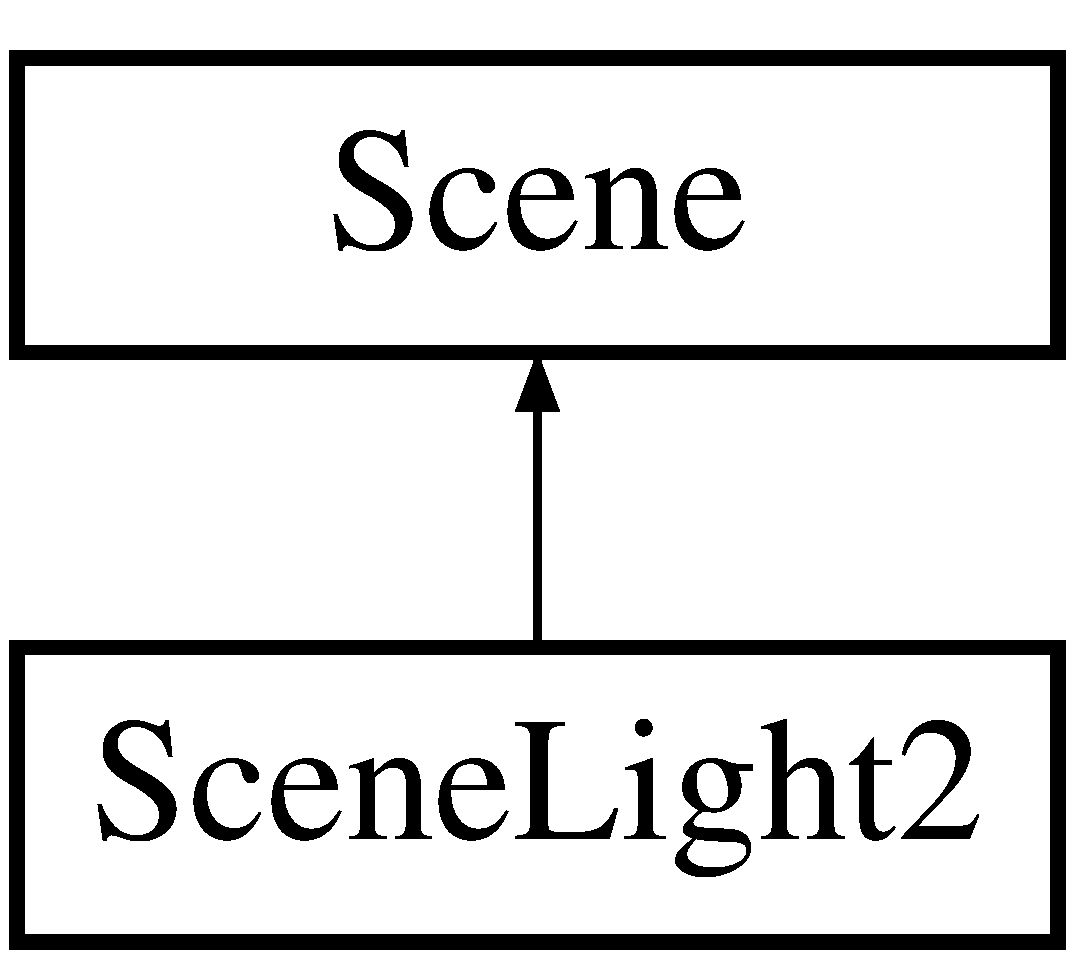
\includegraphics[height=2.000000cm]{class_scene_light2}
\end{center}
\end{figure}
\subsection*{Public Member Functions}
\begin{DoxyCompactItemize}
\item 
\hypertarget{class_scene_light2_acf5ae067a5c4e6b1b212711e12bac1fd}{virtual void {\bfseries Init} ()}\label{class_scene_light2_acf5ae067a5c4e6b1b212711e12bac1fd}

\item 
\hypertarget{class_scene_light2_ae16bbb986e282708b8d867af762f5503}{virtual void {\bfseries Update} (double dt)}\label{class_scene_light2_ae16bbb986e282708b8d867af762f5503}

\item 
\hypertarget{class_scene_light2_a83a2f8226d9ba88e310291f93675bd81}{virtual void {\bfseries Render} ()}\label{class_scene_light2_a83a2f8226d9ba88e310291f93675bd81}

\item 
\hypertarget{class_scene_light2_a4ac35a541882e7c6a4fb58d377e5860d}{virtual void {\bfseries Exit} ()}\label{class_scene_light2_a4ac35a541882e7c6a4fb58d377e5860d}

\item 
\hypertarget{class_scene_light2_a01a8319e888edf26b7657224d2be426c}{void {\bfseries Render\+Body} ()}\label{class_scene_light2_a01a8319e888edf26b7657224d2be426c}

\item 
\hypertarget{class_scene_light2_aeac4f5e4c09818913af9b5e919b4bdd9}{void {\bfseries Render\+Limb} ()}\label{class_scene_light2_aeac4f5e4c09818913af9b5e919b4bdd9}

\item 
\hypertarget{class_scene_light2_ae69b3a73e15b83537879f3a8c4c79797}{void {\bfseries Render\+Robot} ()}\label{class_scene_light2_ae69b3a73e15b83537879f3a8c4c79797}

\item 
\hypertarget{class_scene_light2_ad028e3d047091e6a3a0c02d93bd9d7e5}{void {\bfseries Pikachu\+Left\+Ears} ()}\label{class_scene_light2_ad028e3d047091e6a3a0c02d93bd9d7e5}

\item 
\hypertarget{class_scene_light2_a567f78942a2f0b385cd4ea1a72fefa86}{void {\bfseries Pikachu\+Right\+Ears} ()}\label{class_scene_light2_a567f78942a2f0b385cd4ea1a72fefa86}

\item 
\hypertarget{class_scene_light2_a9e89035ce2a6cd3e3a054adf67a794b1}{void {\bfseries Pikachu\+Head} ()}\label{class_scene_light2_a9e89035ce2a6cd3e3a054adf67a794b1}

\item 
\hypertarget{class_scene_light2_a88811d659896d67c8a52ec7e0b96975a}{void {\bfseries Pikachu\+Right\+Eyes} ()}\label{class_scene_light2_a88811d659896d67c8a52ec7e0b96975a}

\item 
\hypertarget{class_scene_light2_ad143d1b59479c64219d13de05f35f006}{void {\bfseries Pikachu\+Nose} ()}\label{class_scene_light2_ad143d1b59479c64219d13de05f35f006}

\item 
\hypertarget{class_scene_light2_ae5966f852fc393928c3ef0536c6b5ffb}{void {\bfseries Pikachu\+Mouth} ()}\label{class_scene_light2_ae5966f852fc393928c3ef0536c6b5ffb}

\item 
\hypertarget{class_scene_light2_abf145d7167eb753a5ecef20242791a81}{void {\bfseries Pikachu\+Body} ()}\label{class_scene_light2_abf145d7167eb753a5ecef20242791a81}

\item 
\hypertarget{class_scene_light2_a57086f8344bfeee2f870477046adfa7c}{void {\bfseries Pikcahu\+Hands} ()}\label{class_scene_light2_a57086f8344bfeee2f870477046adfa7c}

\item 
\hypertarget{class_scene_light2_ab2ee028987e6b35ed71b8eaae048587f}{void {\bfseries Pikachu\+Left\+Feet} ()}\label{class_scene_light2_ab2ee028987e6b35ed71b8eaae048587f}

\item 
\hypertarget{class_scene_light2_a881484d5b6fc51adc2fcce919cd46f0a}{void {\bfseries Pikachu\+Right\+Feet} ()}\label{class_scene_light2_a881484d5b6fc51adc2fcce919cd46f0a}

\item 
\hypertarget{class_scene_light2_ab39556c22242e92847084ad385b454be}{void {\bfseries Render\+Pikachu} ()}\label{class_scene_light2_ab39556c22242e92847084ad385b454be}

\end{DoxyCompactItemize}


The documentation for this class was generated from the following files\+:\begin{DoxyCompactItemize}
\item 
Scene\+Light2.\+h\item 
Scene\+Light2.\+cpp\end{DoxyCompactItemize}

\hypertarget{class_scene_texture}{\section{Scene\+Texture Class Reference}
\label{class_scene_texture}\index{Scene\+Texture@{Scene\+Texture}}
}
Inheritance diagram for Scene\+Texture\+:\begin{figure}[H]
\begin{center}
\leavevmode
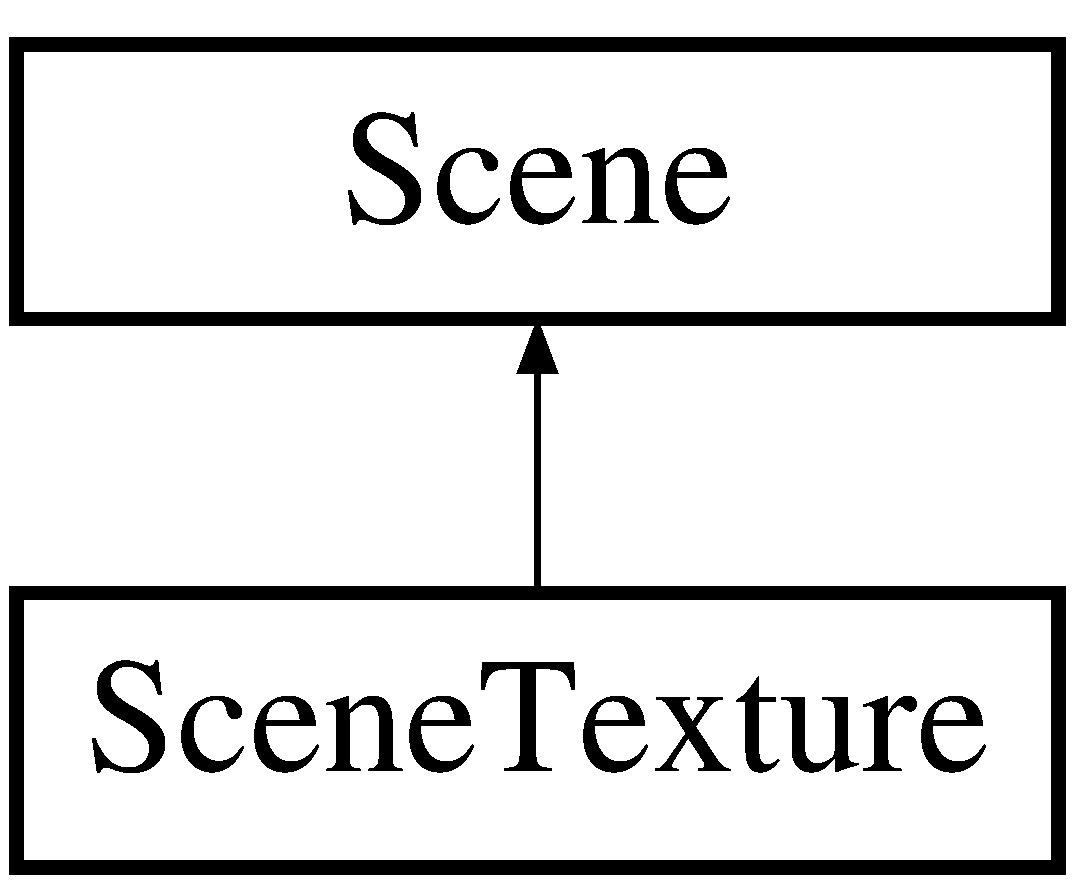
\includegraphics[height=2.000000cm]{class_scene_texture}
\end{center}
\end{figure}
\subsection*{Public Member Functions}
\begin{DoxyCompactItemize}
\item 
\hypertarget{class_scene_texture_a8499b9b84a1509327e29fa5f7899ec58}{virtual void {\bfseries Init} ()}\label{class_scene_texture_a8499b9b84a1509327e29fa5f7899ec58}

\item 
\hypertarget{class_scene_texture_ae7ca4466bb1a3db856c91d714b655253}{virtual void {\bfseries Update} (double dt)}\label{class_scene_texture_ae7ca4466bb1a3db856c91d714b655253}

\item 
\hypertarget{class_scene_texture_ad9009aa06a8d335485a624089ef134f3}{virtual void {\bfseries Render} ()}\label{class_scene_texture_ad9009aa06a8d335485a624089ef134f3}

\item 
\hypertarget{class_scene_texture_aa4771e4c33cef692c7f8520553b680a6}{virtual void {\bfseries Exit} ()}\label{class_scene_texture_aa4771e4c33cef692c7f8520553b680a6}

\end{DoxyCompactItemize}


The documentation for this class was generated from the following files\+:\begin{DoxyCompactItemize}
\item 
Scene\+Texture.\+h\item 
Scene\+Texture.\+cpp\end{DoxyCompactItemize}

\hypertarget{struct_tex_coord}{\section{Tex\+Coord Struct Reference}
\label{struct_tex_coord}\index{Tex\+Coord@{Tex\+Coord}}
}
\subsection*{Public Member Functions}
\begin{DoxyCompactItemize}
\item 
\hypertarget{struct_tex_coord_adec9b45bb816162fe2f22a677ebfc11c}{{\bfseries Tex\+Coord} (float u=0, float v=0)}\label{struct_tex_coord_adec9b45bb816162fe2f22a677ebfc11c}

\item 
\hypertarget{struct_tex_coord_a64b4ceeb1733c478cb4b5b1216146c32}{void {\bfseries Set} (float u, float v)}\label{struct_tex_coord_a64b4ceeb1733c478cb4b5b1216146c32}

\end{DoxyCompactItemize}
\subsection*{Public Attributes}
\begin{DoxyCompactItemize}
\item 
\hypertarget{struct_tex_coord_a3be8371ac57f9ddc6ff5853e4bb58190}{float {\bfseries u}}\label{struct_tex_coord_a3be8371ac57f9ddc6ff5853e4bb58190}

\item 
\hypertarget{struct_tex_coord_ad525bc2c53d6402267c51022db33f85e}{float {\bfseries v}}\label{struct_tex_coord_ad525bc2c53d6402267c51022db33f85e}

\end{DoxyCompactItemize}


The documentation for this struct was generated from the following file\+:\begin{DoxyCompactItemize}
\item 
Vertex.\+h\end{DoxyCompactItemize}

\hypertarget{struct_vertex}{\section{Vertex Struct Reference}
\label{struct_vertex}\index{Vertex@{Vertex}}
}
\subsection*{Public Attributes}
\begin{DoxyCompactItemize}
\item 
\hypertarget{struct_vertex_a8791e77df49f6996a19a8dd17cee8d5c}{\hyperlink{struct_position}{Position} {\bfseries pos}}\label{struct_vertex_a8791e77df49f6996a19a8dd17cee8d5c}

\item 
\hypertarget{struct_vertex_a3a3ff3f6cf46b1848795991e8159b922}{\hyperlink{struct_color}{Color} {\bfseries color}}\label{struct_vertex_a3a3ff3f6cf46b1848795991e8159b922}

\item 
\hypertarget{struct_vertex_adce2d4b3d1191c69328519bdf231c344}{Vector3 {\bfseries normal}}\label{struct_vertex_adce2d4b3d1191c69328519bdf231c344}

\end{DoxyCompactItemize}


The documentation for this struct was generated from the following file\+:\begin{DoxyCompactItemize}
\item 
Vertex.\+h\end{DoxyCompactItemize}

\chapter{File Documentation}
\hypertarget{_mesh_builder_8cpp}{\section{Mesh\+Builder.\+cpp File Reference}
\label{_mesh_builder_8cpp}\index{Mesh\+Builder.\+cpp@{Mesh\+Builder.\+cpp}}
}


\hyperlink{_mesh_builder_8cpp}{Mesh\+Builder.\+cpp} is used to create the V\+B\+O and I\+B\+O of all primitive shapes.  


{\ttfamily \#include \char`\"{}Mesh\+Builder.\+h\char`\"{}}\\*
{\ttfamily \#include $<$G\+L\textbackslash{}glew.\+h$>$}\\*
{\ttfamily \#include $<$vector$>$}\\*
{\ttfamily \#include \char`\"{}Vertex.\+h\char`\"{}}\\*
{\ttfamily \#include \char`\"{}My\+Math.\+h\char`\"{}}\\*
\subsection*{Functions}
\begin{DoxyCompactItemize}
\item 
float \hyperlink{_mesh_builder_8cpp_a42b85724173510abff8489cfe7806c3f}{sphere\+X} (float phi, float theta)
\begin{DoxyCompactList}\small\item\em Calculate the x coordinate of the sphere then return the value back to Generate\+Sphere. \end{DoxyCompactList}\item 
float \hyperlink{_mesh_builder_8cpp_aca2515071d8156673cfaa4b54ae0a558}{sphere\+Y} (float phi, float theta)
\begin{DoxyCompactList}\small\item\em Calculate the y coordinate of the sphere then return the value back to Generate\+Sphere. \end{DoxyCompactList}\item 
float \hyperlink{_mesh_builder_8cpp_ad611a1f30697cb26b310c16a493d8c4f}{sphere\+Z} (float phi, float theta)
\begin{DoxyCompactList}\small\item\em Calculate the z coordinate of the sphere then return the value back to Generate\+Sphere. \end{DoxyCompactList}\item 
float \hyperlink{_mesh_builder_8cpp_a24fc248c98b03e00ffe134f22b9bd16c}{Cylinder\+X} (float theta)
\begin{DoxyCompactList}\small\item\em Calculate calculate radian of theta for the x axis before returning it to Generate\+Cylinder. \end{DoxyCompactList}\item 
float \hyperlink{_mesh_builder_8cpp_a53f49c180979818c704feab0d772ccc0}{Cylinder\+Z} (float theta)
\begin{DoxyCompactList}\small\item\em Calculate calculate radian of theta for the z axis before returning it to Generate\+Cylinder. \end{DoxyCompactList}\end{DoxyCompactItemize}


\subsection{Detailed Description}
\hyperlink{_mesh_builder_8cpp}{Mesh\+Builder.\+cpp} is used to create the V\+B\+O and I\+B\+O of all primitive shapes. 

\begin{DoxyAuthor}{Author}
Ong Swee Seng 
\end{DoxyAuthor}


\subsection{Function Documentation}
\hypertarget{_mesh_builder_8cpp_a24fc248c98b03e00ffe134f22b9bd16c}{\index{Mesh\+Builder.\+cpp@{Mesh\+Builder.\+cpp}!Cylinder\+X@{Cylinder\+X}}
\index{Cylinder\+X@{Cylinder\+X}!Mesh\+Builder.\+cpp@{Mesh\+Builder.\+cpp}}
\subsubsection[{Cylinder\+X}]{\setlength{\rightskip}{0pt plus 5cm}float Cylinder\+X (
\begin{DoxyParamCaption}
\item[{float}]{theta}
\end{DoxyParamCaption}
)}}\label{_mesh_builder_8cpp_a24fc248c98b03e00ffe134f22b9bd16c}


Calculate calculate radian of theta for the x axis before returning it to Generate\+Cylinder. 


\begin{DoxyParams}{Parameters}
{\em theta} & -\/ value of theta\\
\hline
\end{DoxyParams}
\begin{DoxyReturn}{Returns}
x coordinates back to Generate\+Cylinder 
\end{DoxyReturn}
\hypertarget{_mesh_builder_8cpp_a53f49c180979818c704feab0d772ccc0}{\index{Mesh\+Builder.\+cpp@{Mesh\+Builder.\+cpp}!Cylinder\+Z@{Cylinder\+Z}}
\index{Cylinder\+Z@{Cylinder\+Z}!Mesh\+Builder.\+cpp@{Mesh\+Builder.\+cpp}}
\subsubsection[{Cylinder\+Z}]{\setlength{\rightskip}{0pt plus 5cm}float Cylinder\+Z (
\begin{DoxyParamCaption}
\item[{float}]{theta}
\end{DoxyParamCaption}
)}}\label{_mesh_builder_8cpp_a53f49c180979818c704feab0d772ccc0}


Calculate calculate radian of theta for the z axis before returning it to Generate\+Cylinder. 


\begin{DoxyParams}{Parameters}
{\em theta} & -\/ value of theta\\
\hline
\end{DoxyParams}
\begin{DoxyReturn}{Returns}
z coordinates back to Generate\+Cylinder 
\end{DoxyReturn}
\hypertarget{_mesh_builder_8cpp_a42b85724173510abff8489cfe7806c3f}{\index{Mesh\+Builder.\+cpp@{Mesh\+Builder.\+cpp}!sphere\+X@{sphere\+X}}
\index{sphere\+X@{sphere\+X}!Mesh\+Builder.\+cpp@{Mesh\+Builder.\+cpp}}
\subsubsection[{sphere\+X}]{\setlength{\rightskip}{0pt plus 5cm}float sphere\+X (
\begin{DoxyParamCaption}
\item[{float}]{phi, }
\item[{float}]{theta}
\end{DoxyParamCaption}
)}}\label{_mesh_builder_8cpp_a42b85724173510abff8489cfe7806c3f}


Calculate the x coordinate of the sphere then return the value back to Generate\+Sphere. 


\begin{DoxyParams}{Parameters}
{\em theta} & -\/ value of theta \\
\hline
{\em phi} & -\/ value of phi\\
\hline
\end{DoxyParams}
\begin{DoxyReturn}{Returns}
x coordinates back to Generate\+Sphere 
\end{DoxyReturn}
\hypertarget{_mesh_builder_8cpp_aca2515071d8156673cfaa4b54ae0a558}{\index{Mesh\+Builder.\+cpp@{Mesh\+Builder.\+cpp}!sphere\+Y@{sphere\+Y}}
\index{sphere\+Y@{sphere\+Y}!Mesh\+Builder.\+cpp@{Mesh\+Builder.\+cpp}}
\subsubsection[{sphere\+Y}]{\setlength{\rightskip}{0pt plus 5cm}float sphere\+Y (
\begin{DoxyParamCaption}
\item[{float}]{phi, }
\item[{float}]{theta}
\end{DoxyParamCaption}
)}}\label{_mesh_builder_8cpp_aca2515071d8156673cfaa4b54ae0a558}


Calculate the y coordinate of the sphere then return the value back to Generate\+Sphere. 


\begin{DoxyParams}{Parameters}
{\em theta} & -\/ value of theta \\
\hline
{\em phi} & -\/ value of phi\\
\hline
\end{DoxyParams}
\begin{DoxyReturn}{Returns}
y coordinates back to Generate\+Sphere 
\end{DoxyReturn}
\hypertarget{_mesh_builder_8cpp_ad611a1f30697cb26b310c16a493d8c4f}{\index{Mesh\+Builder.\+cpp@{Mesh\+Builder.\+cpp}!sphere\+Z@{sphere\+Z}}
\index{sphere\+Z@{sphere\+Z}!Mesh\+Builder.\+cpp@{Mesh\+Builder.\+cpp}}
\subsubsection[{sphere\+Z}]{\setlength{\rightskip}{0pt plus 5cm}float sphere\+Z (
\begin{DoxyParamCaption}
\item[{float}]{phi, }
\item[{float}]{theta}
\end{DoxyParamCaption}
)}}\label{_mesh_builder_8cpp_ad611a1f30697cb26b310c16a493d8c4f}


Calculate the z coordinate of the sphere then return the value back to Generate\+Sphere. 


\begin{DoxyParams}{Parameters}
{\em theta} & -\/ value of theta \\
\hline
{\em phi} & -\/ value of phi\\
\hline
\end{DoxyParams}
\begin{DoxyReturn}{Returns}
z coordinates back to Generate\+Sphere 
\end{DoxyReturn}

\hypertarget{_scene_light_8cpp}{\section{Scene\+Light.\+cpp File Reference}
\label{_scene_light_8cpp}\index{Scene\+Light.\+cpp@{Scene\+Light.\+cpp}}
}


\hyperlink{_scene_light_8cpp}{Scene\+Light.\+cpp} is used to set, render and update geometries with parameters.  


{\ttfamily \#include \char`\"{}Scene\+Light.\+h\char`\"{}}\\*
{\ttfamily \#include \char`\"{}G\+L\textbackslash{}glew.\+h\char`\"{}}\\*
{\ttfamily \#include \char`\"{}shader.\+hpp\char`\"{}}\\*
{\ttfamily \#include \char`\"{}Mtx44.\+h\char`\"{}}\\*
{\ttfamily \#include \char`\"{}Utility.\+h\char`\"{}}\\*
{\ttfamily \#include \char`\"{}Application.\+h\char`\"{}}\\*
{\ttfamily \#include \char`\"{}Mesh\+Builder.\+h\char`\"{}}\\*


\subsection{Detailed Description}
\hyperlink{_scene_light_8cpp}{Scene\+Light.\+cpp} is used to set, render and update geometries with parameters. 

\begin{DoxyAuthor}{Author}
Ong Swee Seng 
\end{DoxyAuthor}

%--- End generated contents ---

% Index
\newpage
\phantomsection
\addcontentsline{toc}{chapter}{Index}
\printindex

\end{document}
